% !TEX root = ../thesis-sample.tex

\chapter{Experimental Results}\label{chap:Experiments}

In this chapter, we present three experiments that demonstrate the efficacy of the proposed exact occupancy grid mapping and autonomous exploration from earlier chapters. The first example involves a ground vehicle mapping and exploring a 2D space. The second example is a quadrotor unmanned aerial vehicle (UAV) flying around a vertically-uniform space while generating a 3D map from level flight. The final example shows autonomous exploration completely in 3D, where a quadrotor must map and explore around complicated objects.

\section{Pioneer Ground Vehicle Tests}
\label{sec:PioneerNRL}

The experiment involves a ground vehicle producing a probabilistic occupancy grid map in real time. The robot motion is governed by the information gain-maximizing policy described in Chapter \ref{chap:ae2D}.


\subsection{Hardware Configuration}
The Pioneer 3 ground robot is chosen for this experiment because of its reliability and simple operation. The vehicle accepts two inputs, namely linear velocity (aligned with the robot wheels) and angular velocity (about a central axis passing vertically through the robot). The robot pose is estimated via Vicon Tracker, which provides the location and attitude of a rigid body. The depth readings are obtained by a Kinect depth sensor. Since the experiment is to map and explore a 2D environment, only a single central row of the 3D Kinect depth scan provide the necessary measurements. The robot captures an experimental environment with walls constructed from Styrofoam.

\subsection{Software Configuration}

The software structure is similar to ROS nodes Section \ref{sec:Ae2DNumExamples}, which simply involves a mapping node, an exploration node, and a visualization node using ``OpenGL'' libraries. The only differences are eliminating the simulator (Stage) and adding synchronization among the sensors, which is of high importance to the proposed occupancy grid mapping approach. Any time delay between the robot pose estimation and the sensor depth readings can cause conflicting information, which may be harmful to the probabilistic map. Thus, ROS approximate message filters are applied such that the pose from Vicon Tracker ($100$Hz) and the Microsoft Kinect ($30$Hz) are nearly synchronized, which provides validity of the assumption that the measurement ray positions and directions are known deterministically.

\subsection{Exploring and Mapping a 2D Environment}
The environment consists of Styrofoam walls on a flat floor. The perimeter is rectangular, with several obstacles and angled walls (see Figure \ref{fig:ExpSetupPhoto}). The robot autonomously explored the space using the complete Cartesian searching approach, and Dijkstra's algorithm provides collision-free waypoints to the optimal future poses. Based on these waypoints, a constrained least squares polynomial fitting generates a smooth trajectory to follow the waypoints with fixed velocity. Finally, a simple controller is implemented such that the Pioneer follows the trajectory by moving and orienting toward the desired robot location $1$ sec in the future.

\begin{figure}
	\centering
    	\begin{subfigure}[b]{0.45\textwidth}
        		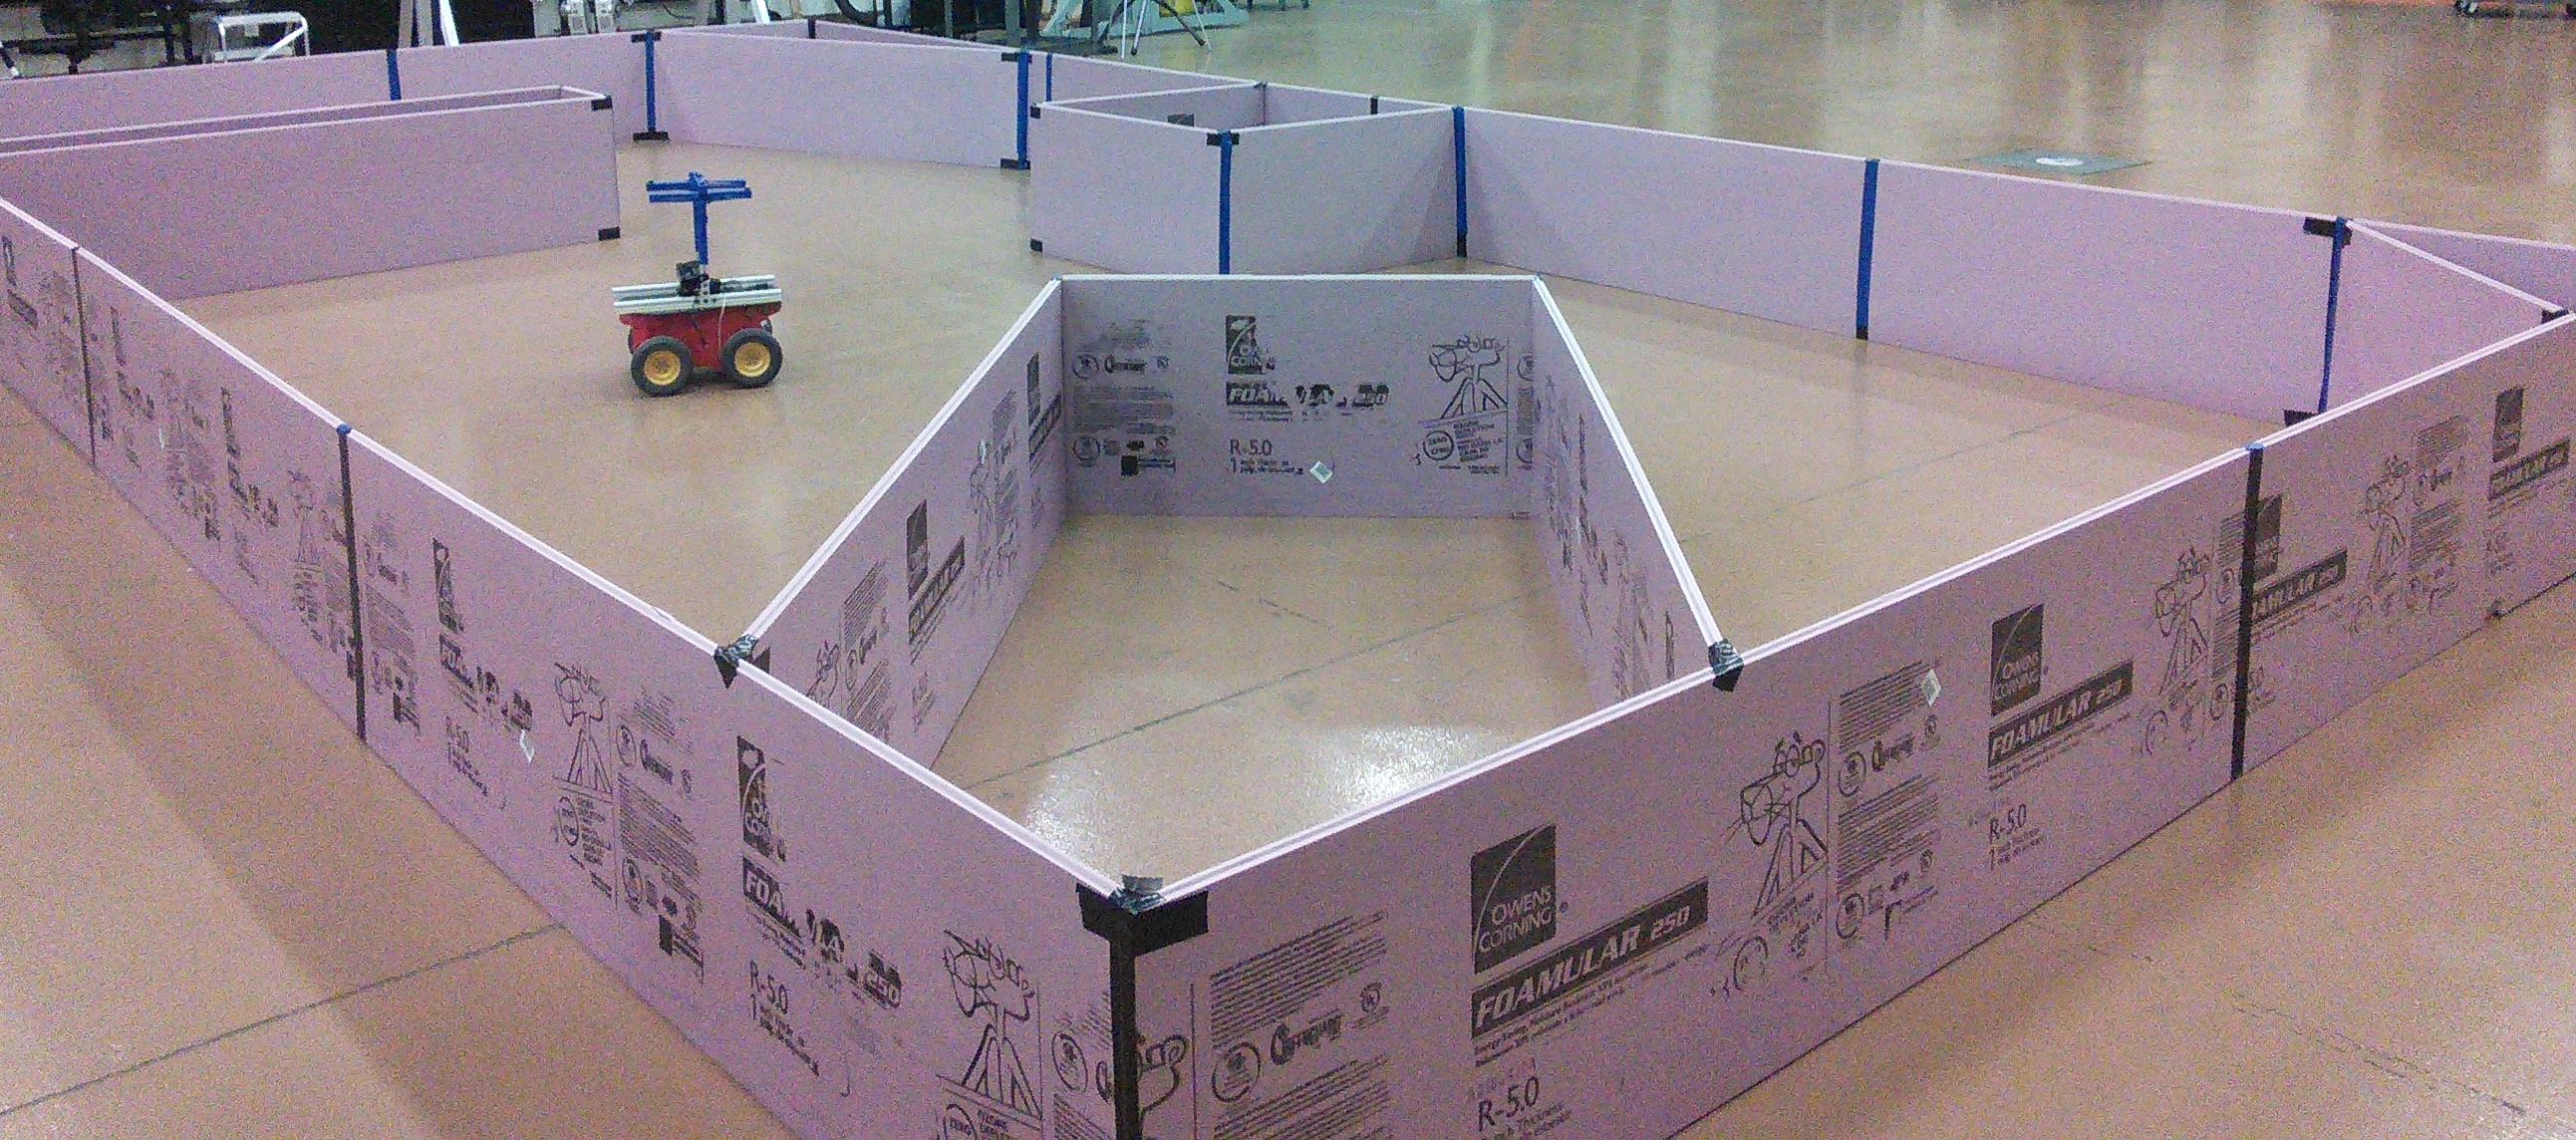
\includegraphics[width=\textwidth]{test_setup_bottom_left_cropped.jpg}
        		\caption{Bottom-left view}
        		\label{fig:Experiment_blv}
    	\end{subfigure}
	\hspace*{0.05\columnwidth}
	\begin{subfigure}[b]{0.45\textwidth}
        		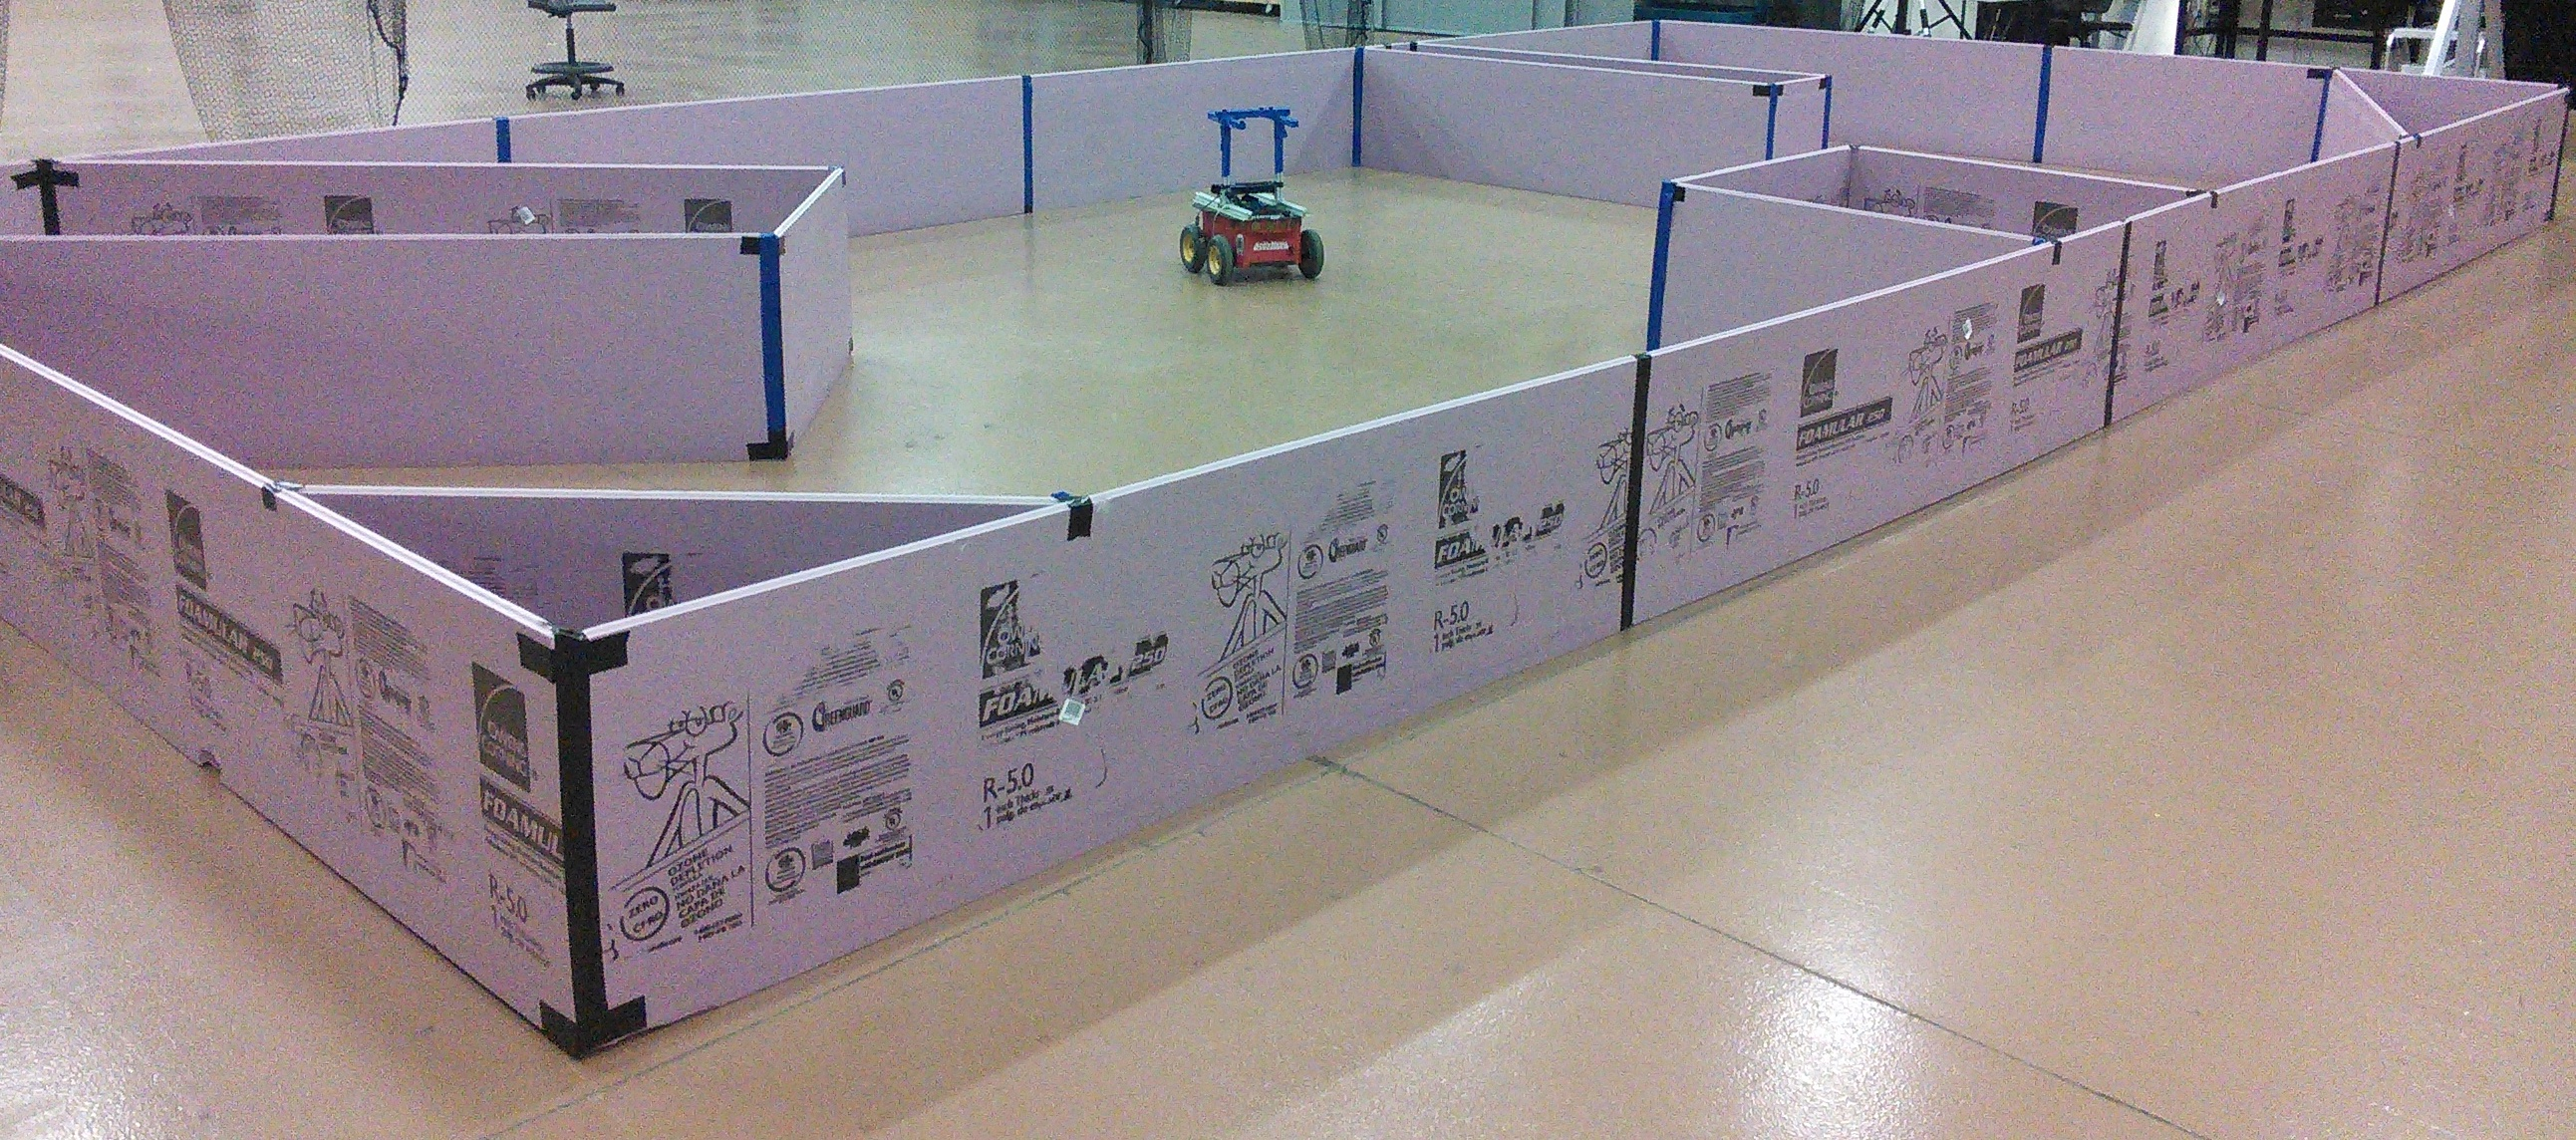
\includegraphics[width=\textwidth]{test_setup_bottom_right_cropped.jpg}
        		\caption{Bottom-right view}
        		\label{fig:Experiment_brv}
    	\end{subfigure}
\caption{2D Experimental Environment}
	\medskip
	\small
	Images from two perspectives show the walls and obstacles of the experimental environment.
\label{fig:ExpSetupPhoto}
\end{figure}


The resulting occupancy grid maps and trajectories are depicted in Figure \ref{fig:ExperimentOGM} and a video is available at \href{https://www.youtube.com/watch?v=CRQfhhICSj0&feature=youtu.be}{\WriteBlue{www.youtube.com/watch?v=CRQfhhICSj0\&feature=youtu.be}}. Most importantly, the robot builds a clear occupancy grid map despite sensor noise and imperfect sensor synchronization. The autonomous exploration successfully guides the robot such that it builds a map of the reachable space without colliding with any obstacles.


\begin{figure}
	\centering{
    	\begin{subfigure}[b]{0.19\textwidth}
        		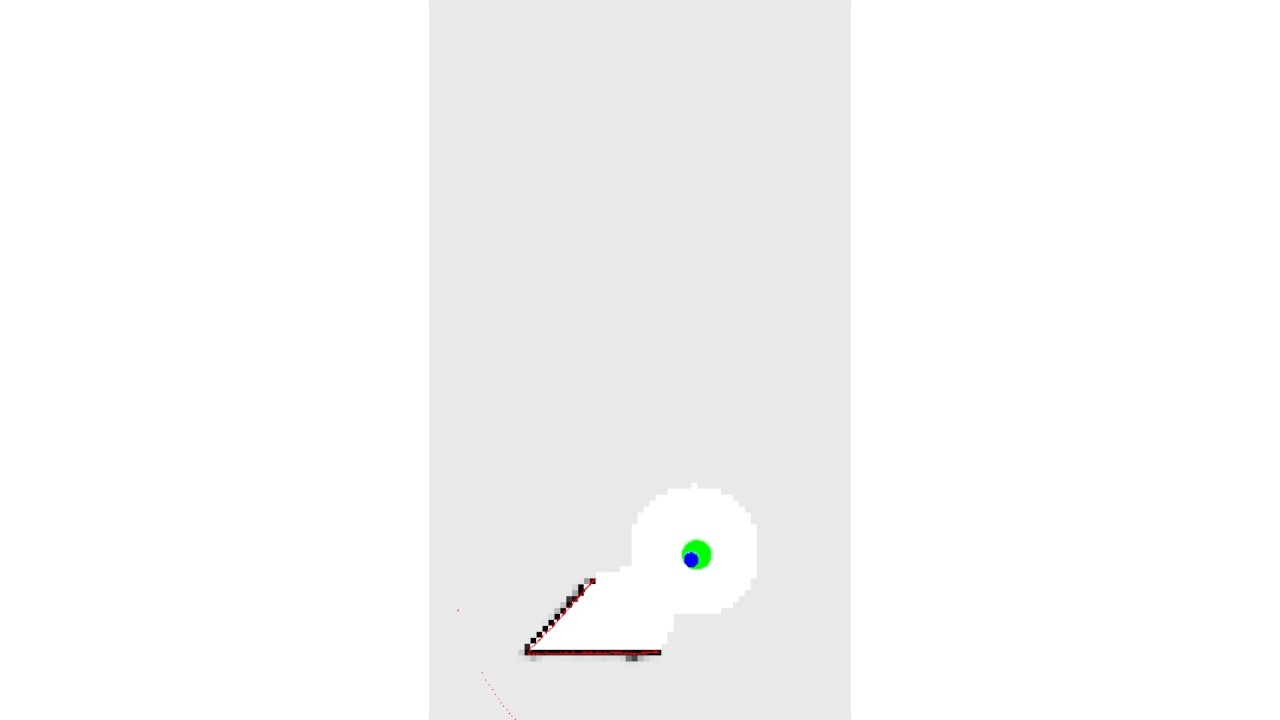
\includegraphics[trim={13cm 1cm 13cm 0}, clip, width=\textwidth]{feb23_t0sec.jpg}
        		\caption{$t=0$ sec}
        		\label{fig:Experiment_ogm_t0}
    	\end{subfigure}
	\begin{subfigure}[b]{0.19\textwidth}
        		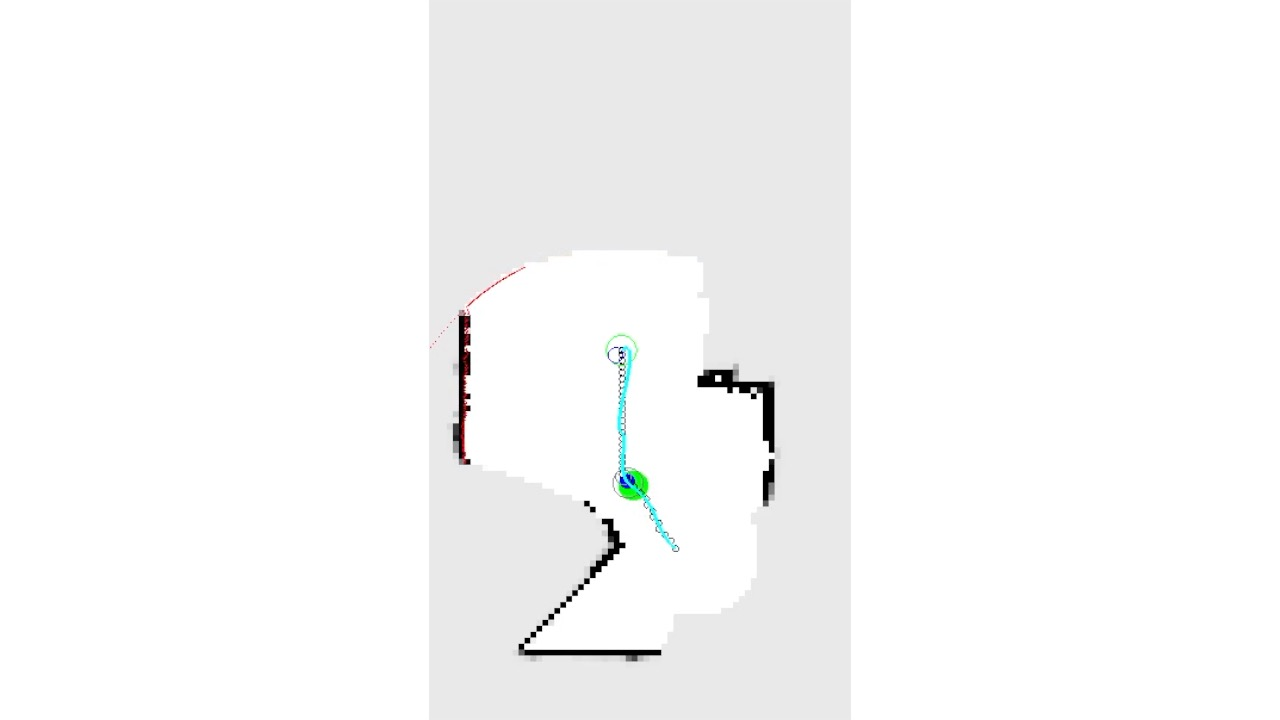
\includegraphics[trim={13cm 1cm 13cm 0}, clip, width=\textwidth]{feb23_t20sec.jpg}
        		\caption{$t=20$ sec}
        		\label{fig:Experiment_ogm_t0p5}
    	\end{subfigure}    
	\begin{subfigure}[b]{0.19\textwidth}
        		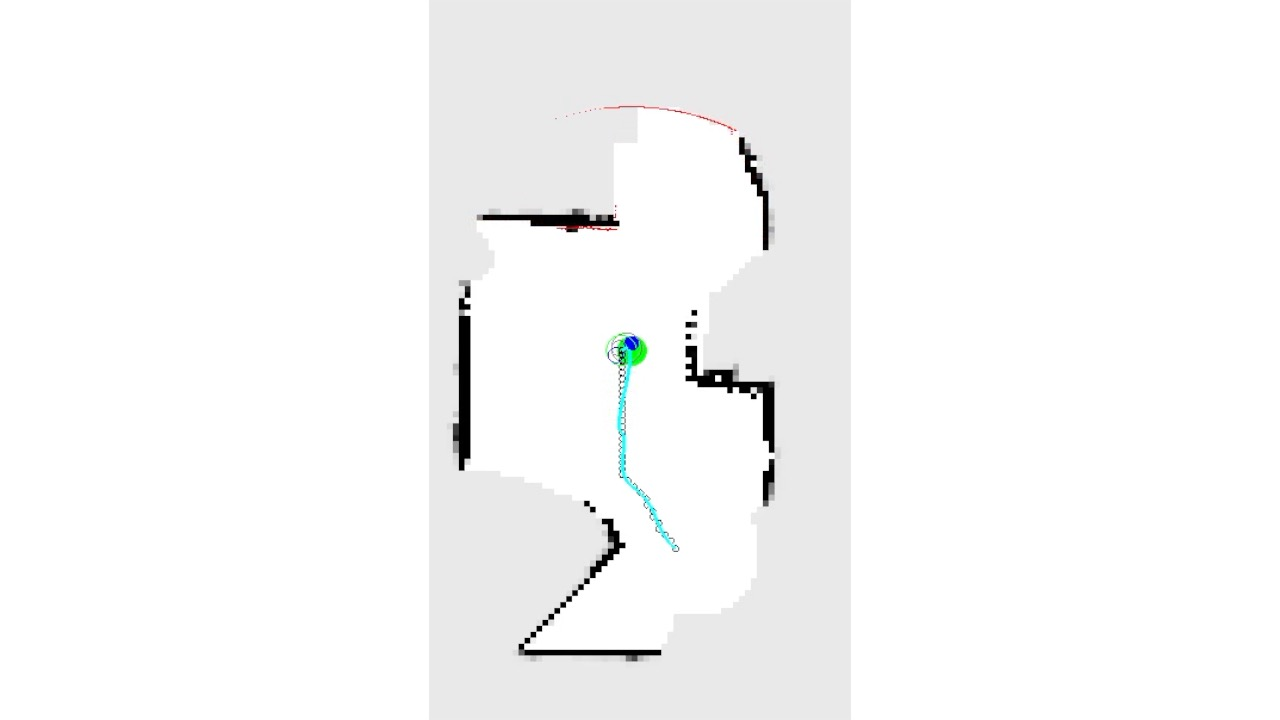
\includegraphics[trim={13cm 1cm 13cm 0}, clip, width=\textwidth]{feb23_t40sec.jpg}
        		\caption{$t=40$ sec}
        		\label{fig:Experiment_ogm_t1}
    	\end{subfigure}
	\begin{subfigure}[b]{0.19\textwidth}
        		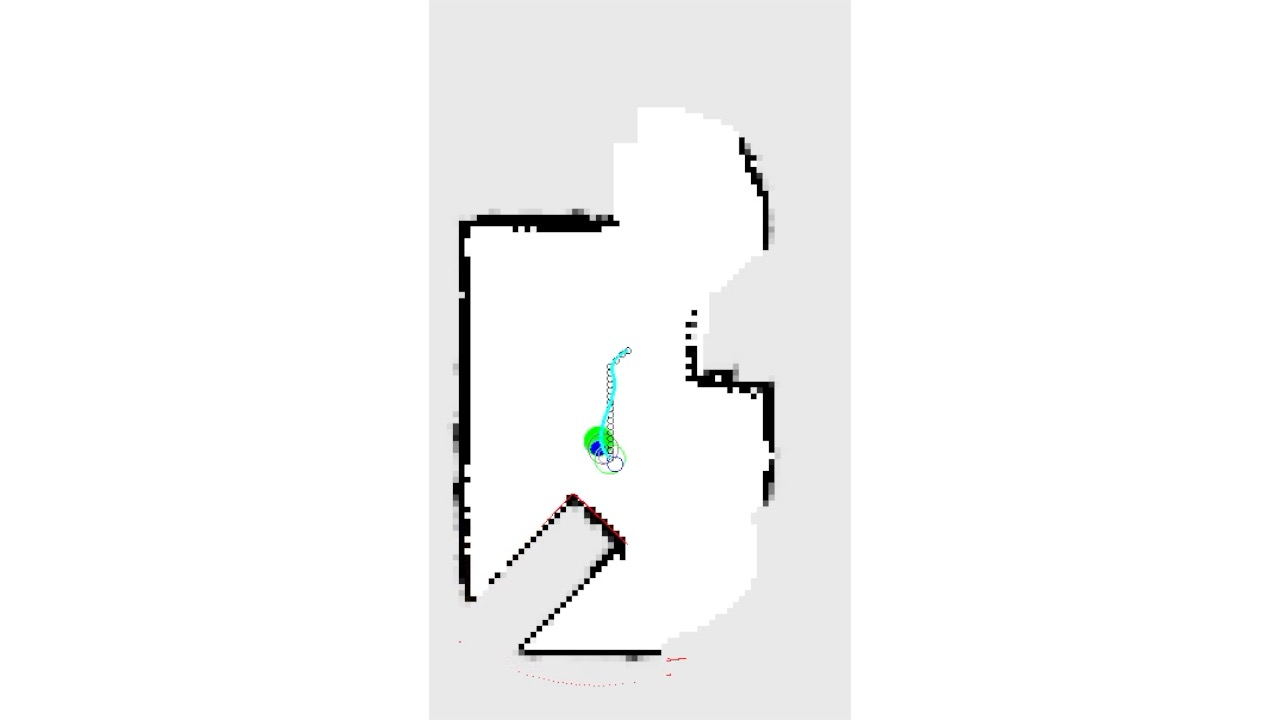
\includegraphics[trim={13cm 1cm 13cm 0}, clip, width=\textwidth]{feb23_t60sec.jpg}
        		\caption{$t=60$ sec}
        		\label{fig:Experiment_ogm_t1p5}
    	\end{subfigure}
	\begin{subfigure}[b]{0.19\textwidth}
        		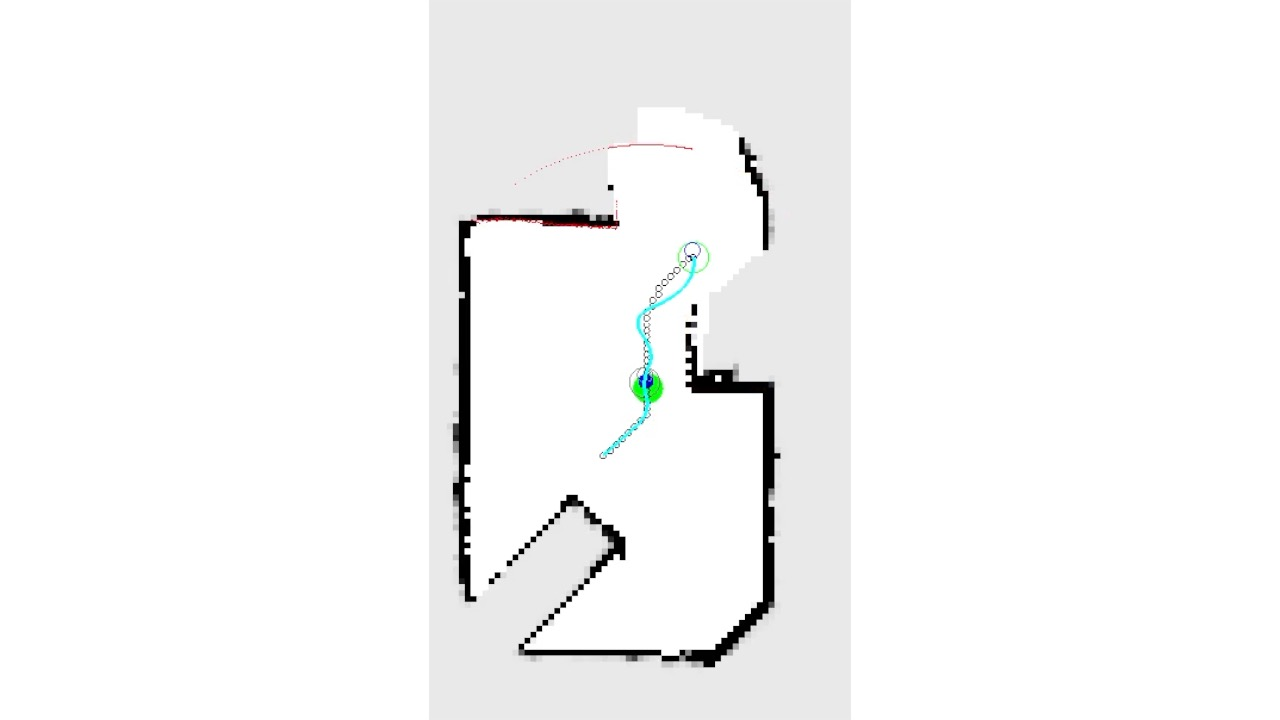
\includegraphics[trim={13cm 1cm 13cm 0}, clip, width=\textwidth]{feb23_t80sec.jpg}
        		\caption{$t=80$ sec}
        		\label{fig:Experiment_ogm_t2}
    	\end{subfigure}
		\vspace*{0.05\textwidth}

	}
	\centering{
    	\begin{subfigure}[b]{0.19\textwidth}
        		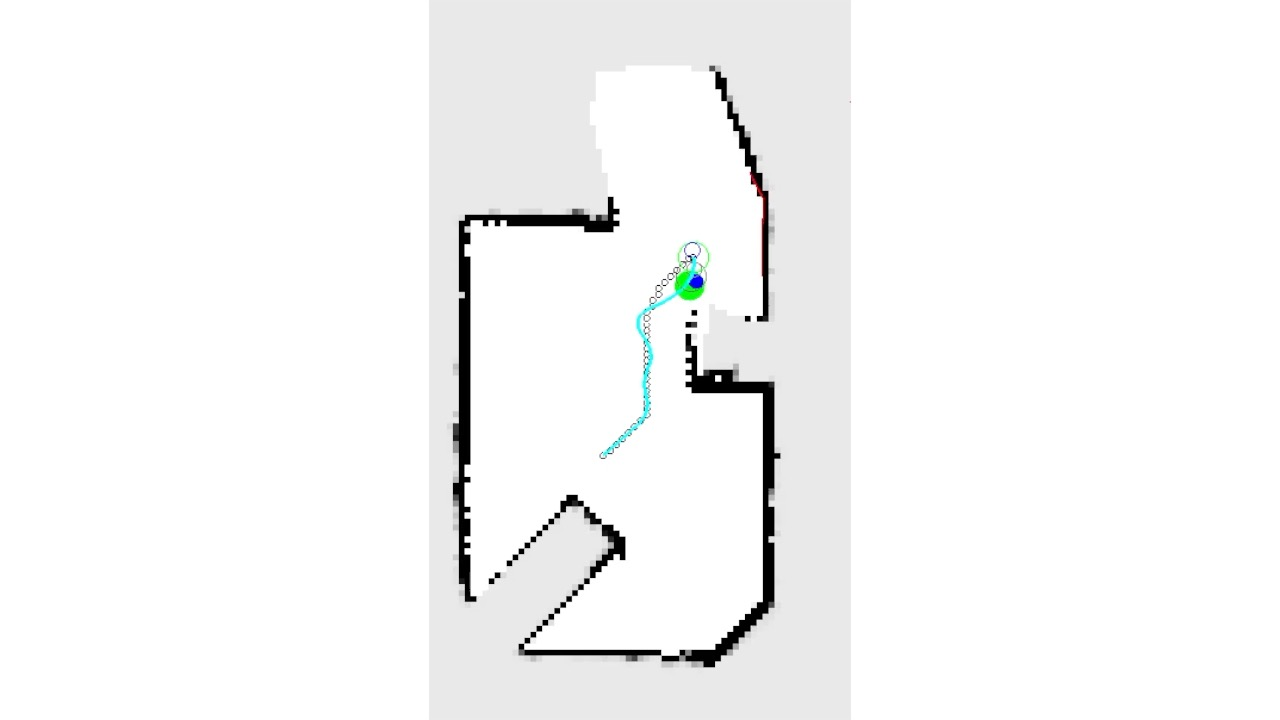
\includegraphics[trim={13cm 1cm 13cm 0}, clip, width=\textwidth]{feb23_t100sec.jpg}
        		\caption{$t=100$ sec}
        		\label{fig:Experiment_ogm_t2p5}
    	\end{subfigure}
	\begin{subfigure}[b]{0.19\textwidth}
        		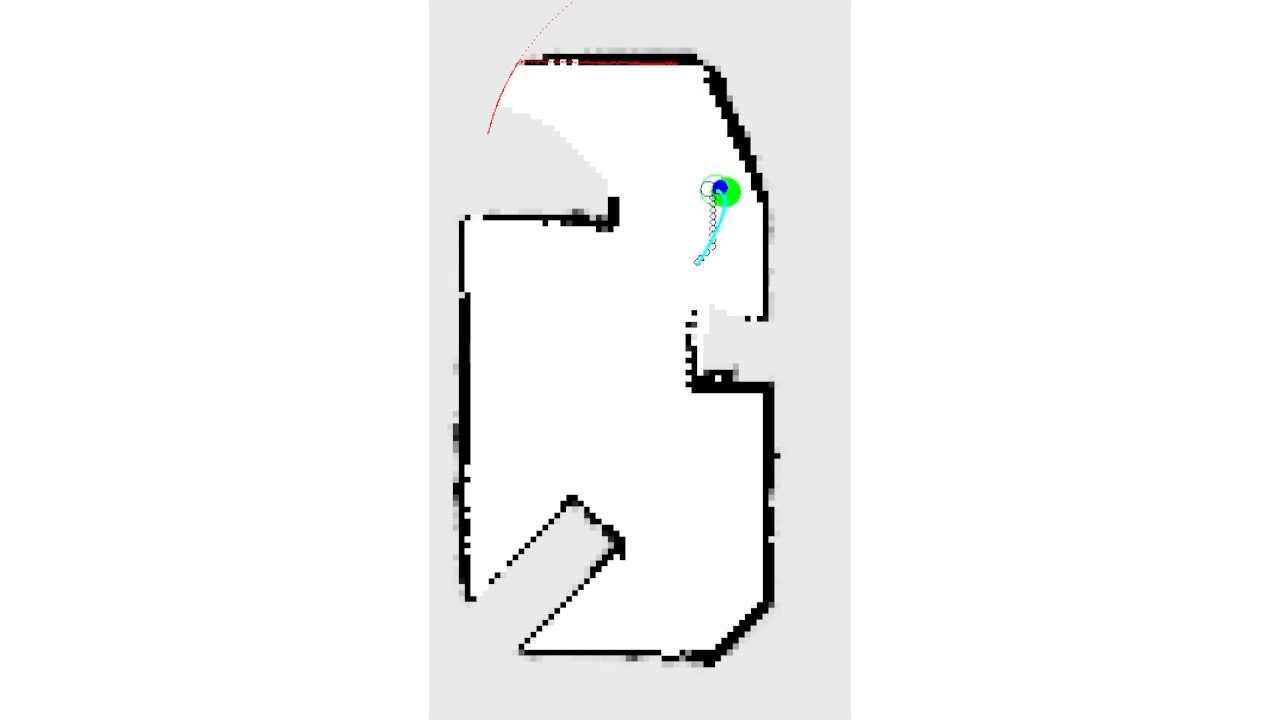
\includegraphics[trim={13cm 1cm 13cm 0}, clip, width=\textwidth]{feb23_t120sec.jpg}
        		\caption{$t=120$ sec}
        		\label{fig:Experiment_ogm_t3}
    	\end{subfigure}    
	\begin{subfigure}[b]{0.19\textwidth}
        		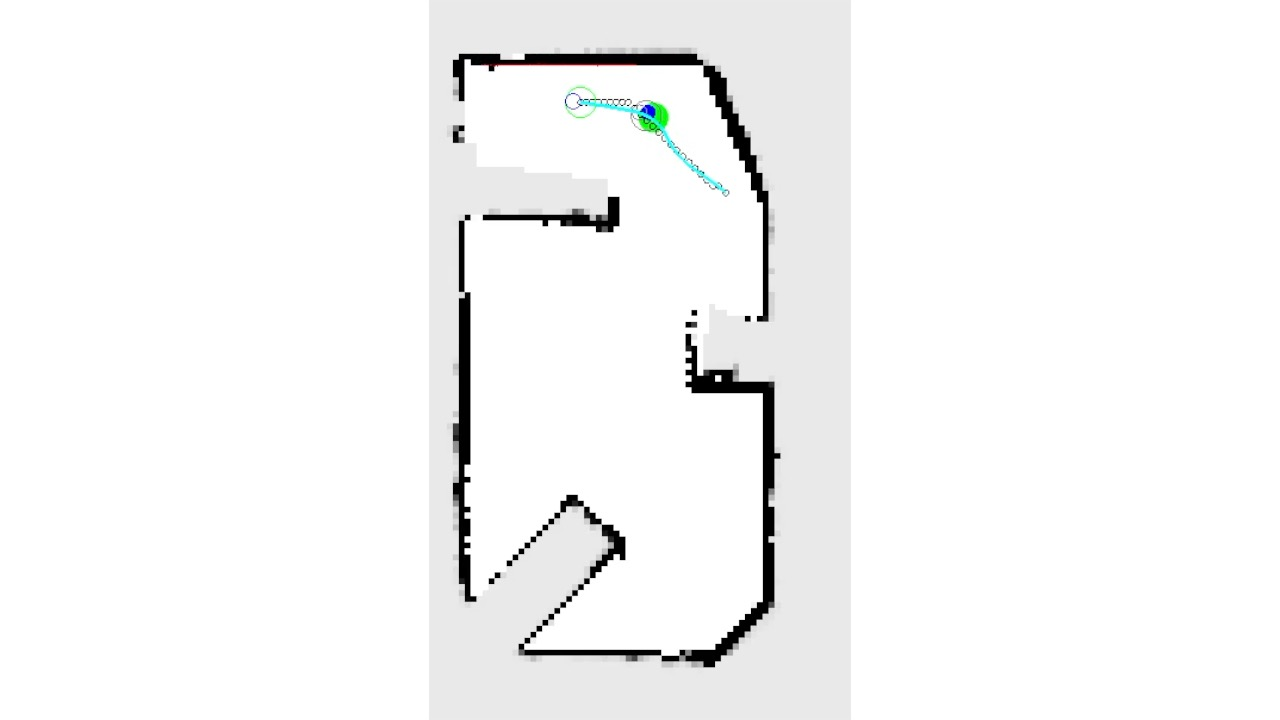
\includegraphics[trim={13cm 1cm 13cm 0}, clip, width=\textwidth]{feb23_t140sec.jpg}
        		\caption{$t=140$ sec}
        		\label{fig:Experiment_ogm_t3p5}
    	\end{subfigure}
	\begin{subfigure}[b]{0.19\textwidth}
        		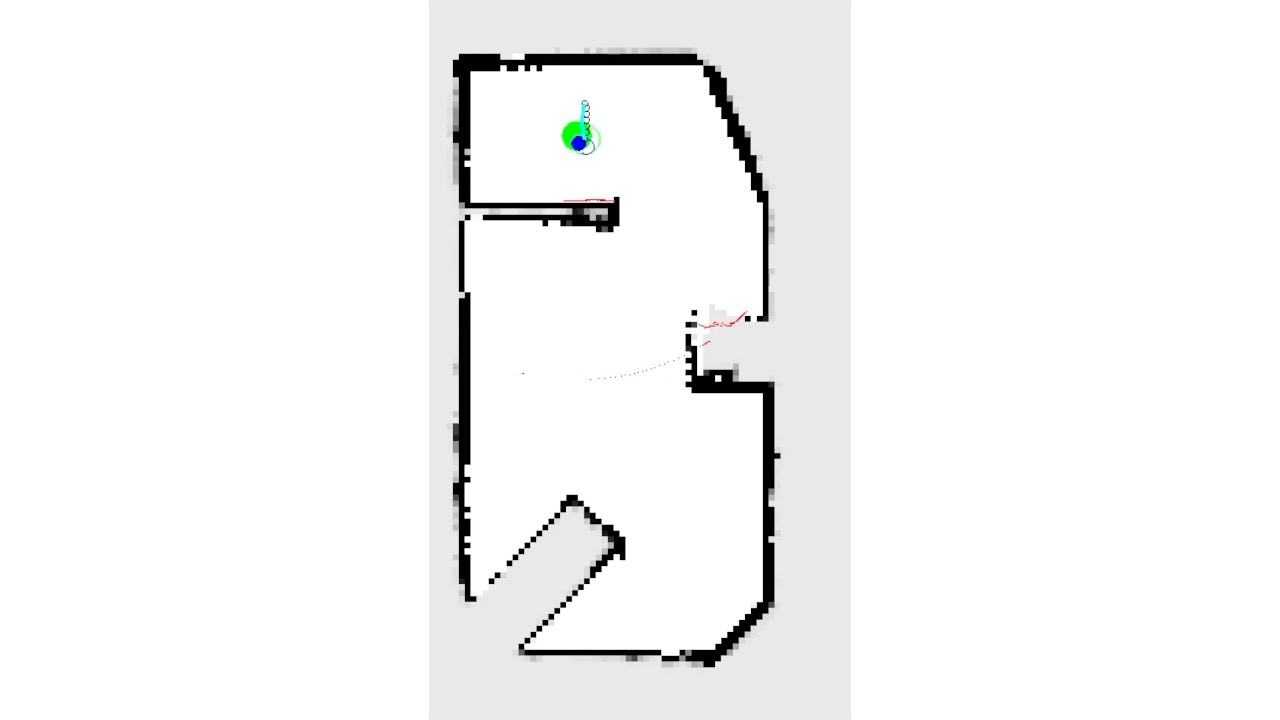
\includegraphics[trim={13cm 1cm 13cm 0}, clip, width=\textwidth]{feb23_t160sec.jpg}
        		\caption{$t=160$ sec}
        		\label{fig:Experiment_ogm_t4}
    	\end{subfigure}
	\begin{subfigure}[b]{0.19\textwidth}
        		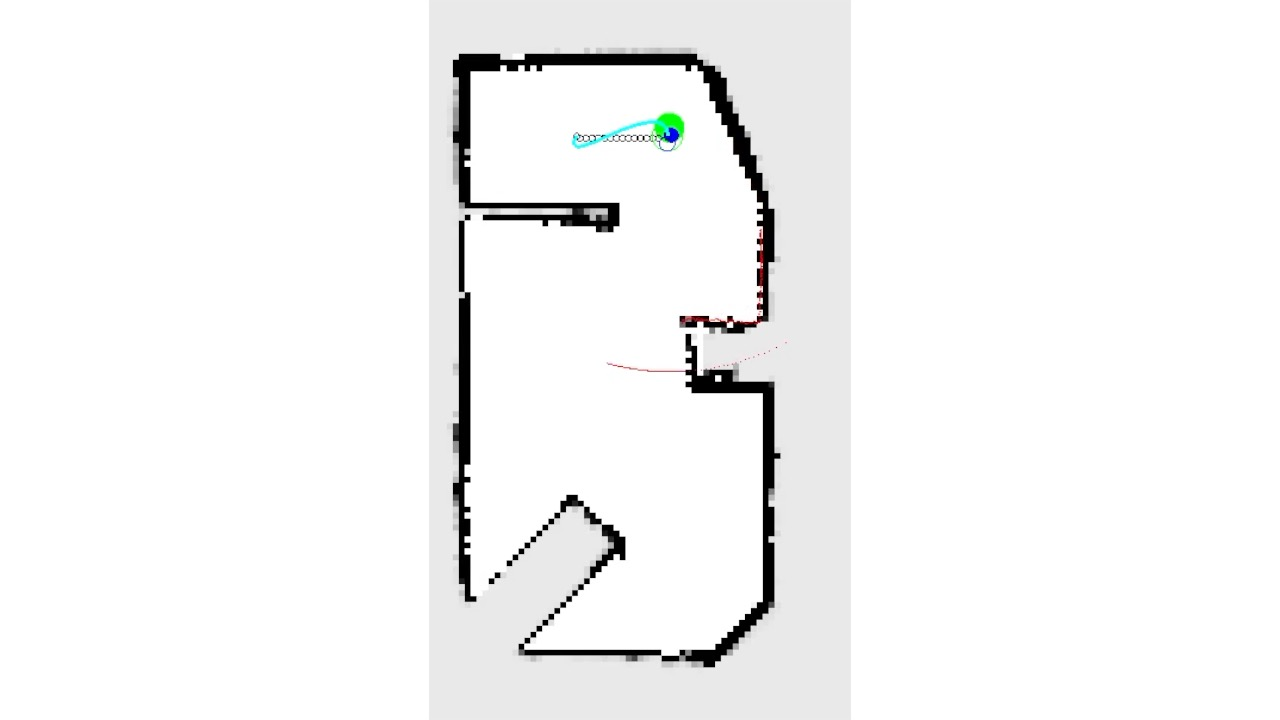
\includegraphics[trim={13cm 1cm 13cm 0}, clip, width=\textwidth]{feb23_t180sec.jpg}
        		\caption{$t=180$ sec}
        		\label{fig:Experiment_ogm_t4p5}
    	\end{subfigure}
	}
\caption{A robot autonomously explores the experimental environment and produces an occupancy grid map along the way. The robot (shaded green circle body with shaded blue circle sensor) is controlled toward the desired pose $1$ sec in the future (unshaded grey robot), which is following a constrained least-squares trajectory (cyan curve). This trajectory is based on waypoints (black circles) from Dijkstra's algorithm to arrive at the optimal pose (unshaded green circle body with unshaded blue circle sensor) as proposed in this paper.}
\label{fig:ExperimentOGM}
\end{figure}

The resulting map and exploration commands are generated in real time. The grid cells are stored as double-float variables in a vector, where the vector index is mapped to a location on the occupancy grid. Thus, the memory requirements are proportional to the number of grid cells, which is roughly the mapping area divided by the area of a grid cell. Since cell locations need not be saved because the mapping between cell index and location is known, memory requirements are reduced. On a Lenovo T540p laptop with an Intel Core i7-4900MQ processor (quad-core, 2.8GHz per core) and 16GB of RAM, the mean time for updating the occupancy grid is $0.0115$ seconds, and the mean time to determine an exploration strategy is $0.6820$ seconds. Time requirements for mapping and exploration are easily modified by changing grid cell resolution or the number of exploration pose candidates, respectively. In short, there is a tradeoff between computational speed and accuracy of mapping or exploration.

The autonomous exploration is governed by a policy to maximize expected entropy decreases, so entropy and entropy change with time (Figure \ref{fig:ExperimentH}) are important metrics. In this example, the a priori occupancy probabilities of all cells are $0.1$, so the entropies could temporarily rise for likely occupied cells. The total map entropy begins at roughly $2613$ and decreases by roughly half to $1338$. Many grid cells within the map limits are occluded by walls, preventing the blocked cells from occupancy probability changes. In some cases, the robot is able to update the cell occupancy probabilities; in other cases, cells fall inside regions occluded from all reachable space, and the robot cannot update these cells. Among those grid cells visible from collision-free locations, the vast majority of cells were updated in less than $3$ min while following a very slow ($5$ cm/sec) trajectory.

In conclusion, this example shows how occupancy grid mapping and autonomous exploration are applied to a ground vehicle in a 2D environment such as a floor of a house or building. Dijkstra's search is applied about the occupancy grid, and a smooth trajectory is easily tracked with a simple controller that tracks a polynomial least squares trajectory. These results show the efficacy of exact occupancy grid mapping and autonomous exploration. Next, we extend these experiments to 3D.

\begin{figure}
	\centering
	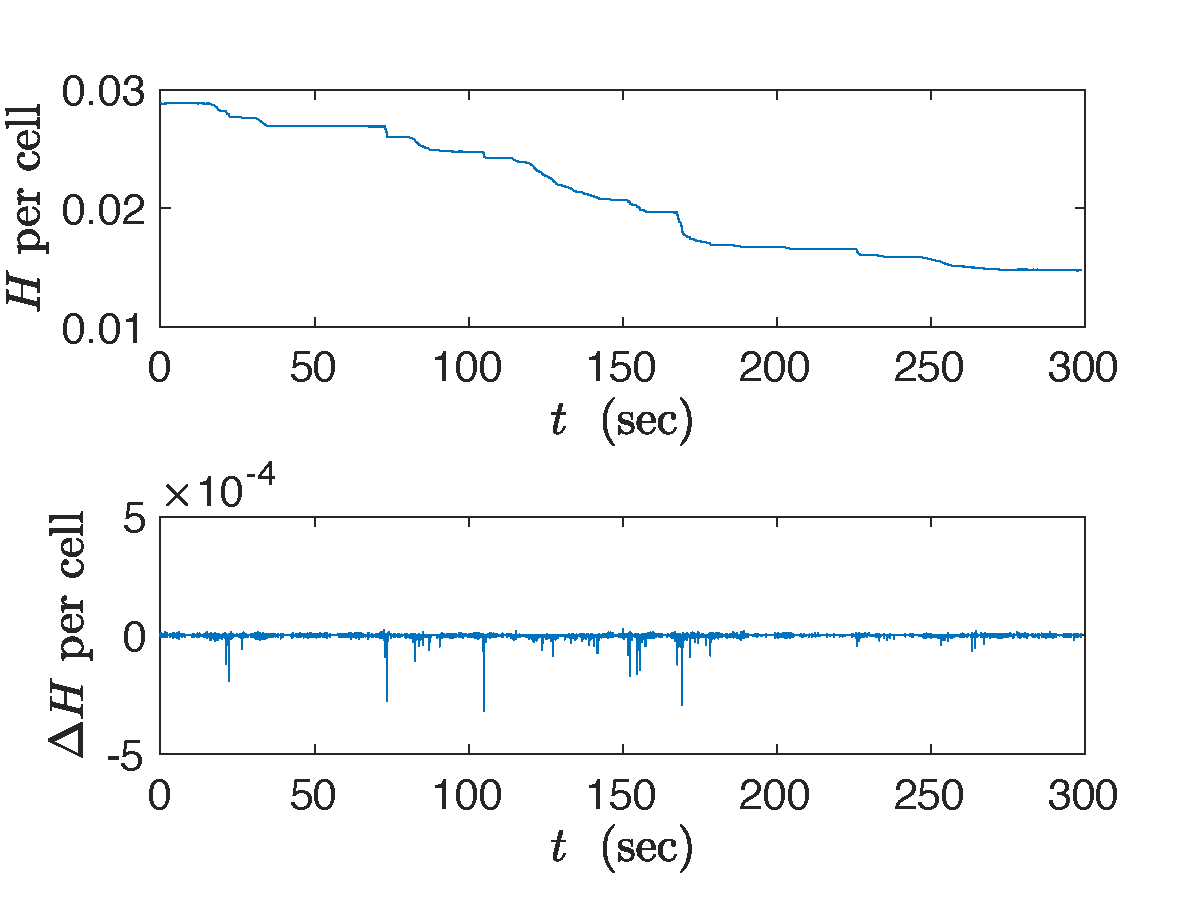
\includegraphics[width=\textwidth]{JIRS_fig11.pdf}
	\caption{The map entropy $H$ averaged over all $90601$ grid cells is reduced during experimentation. The quick changes $\Delta H$ per cell correspond to map updates when the robot captures new territory.}
\label{fig:ExperimentH}
\end{figure}




\section{Quadrotor Exploration of a Large Room}
\label{sec:QuadrotorNRL}


In this section, we present results from a quadrotor as it autonomously explores a nearly vertically-uniform room. A robots builds a 3D map of its environment, which is projected onto a 2D map for exploration following the process described in Section~\ref{sec:MapProjections}. The software structure and sensor parameters are identical to those presented in Section~\ref{sec:Compare2MapProjections}.

\subsection{Exploration Environment}

The U.S. Naval Research Laboratory (NRL) has a large experimental space for testing known as the Laboratory for Autonomous Systems Research (LASR). Here, the experimental setup contains walls and objects to resemble a building floor plan. The perimeter walls are constructed with tan cardboard, which were suspended from $1$ m tall stanchions, and an internal wall is built with gray metal sheeting mounted to $80/20$ supports~\cite{url_8020}. Additionally, a hard flooring reflects some florescent lighting above. The objects inside the experimental environment include various trash cans, desks, and chairs in addition to a few miscellaneous objects. The map size is selected to slightly exceed the volume of the experiment such that the the x-direction (positive east) spans $0.5$ m to $10.3$ m, the y-direction (positive north) spans $-8.3$ m to $3.5$ m, and the z-direction (positive vertically up) spans $-0.15$ m to $1.5$ m. Two images of the experimental environment are displayed in Figure \ref{fig:exp3DEnvironment}.

\begin{figure}[!t]
\centering
    	\begin{subfigure}[t]{0.95\columnwidth}
           	\centering
          	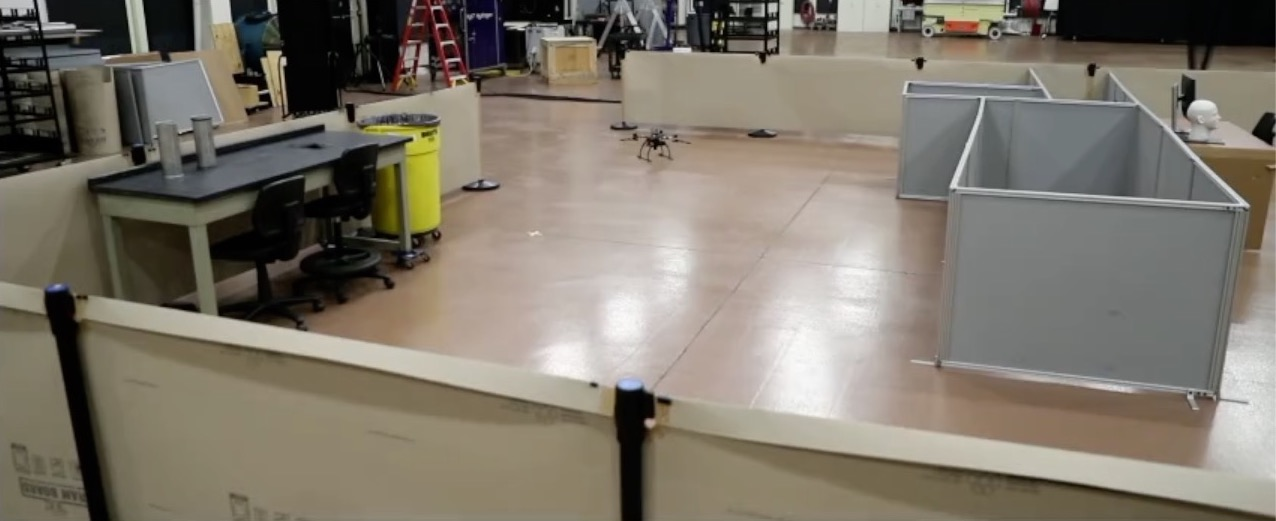
\includegraphics[width=\textwidth]{experiment_north.jpg}
        		\caption{North Region}
    	\end{subfigure}
    	\begin{subfigure}[t]{0.95\columnwidth}
	\vspace*{0.03\columnwidth}
           	\centering
          	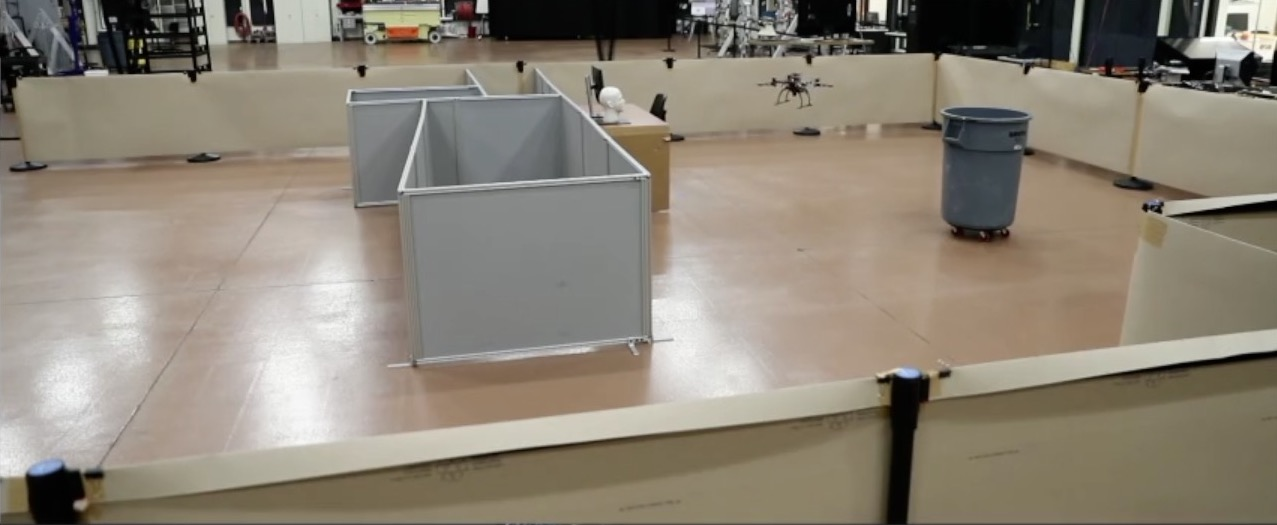
\includegraphics[width=\textwidth]{experiment_south.jpg}
        		\caption{South Region}
    	\end{subfigure}
	\caption{The 3D experimental environment is designed to resemble a large room within an office building. The walls are build from from cardboard suspended from stanchions and gray sheeting with $80/20$ supports, and miscellaneous objects are placed around the room as well.}
	\label{fig:exp3DEnvironment}
\end{figure}


\subsection{Hardware Structure}

Several components are used for localization, sensing, and actuation. A Vicon motion capture system provides the transformation between a reference frame fixed to the world and the moving vehicle. This transformation, along with fixed transformations between the robot body and the sensors, provides sufficient information for the transformation from the world to each sensor frame. The sensor readings from the Xtion and Hokuyo are transmitted from an NVidia Jetson TX2 onboard the vehicle (Figure \ref{fig:QuadrotorHardware}). The sensor readings are received via WIFI on a host computer with an Intel Core i7-6800K CPU (12$\times$3.40GHz), which runs the mapping and exploration nodes. The host computer returns the exploration trajectories to the Jetson TX2 over WIFI. Then, the Jetson executes a nonlinear geometric flight controller~\cite{GooDaeLee13} onboard. With this configuration, large processing tasks are avoided onboard the robot.
		
\begin{figure}[!t]
\centering
    	\begin{subfigure}[t]{0.44\columnwidth}
           	\centering
          	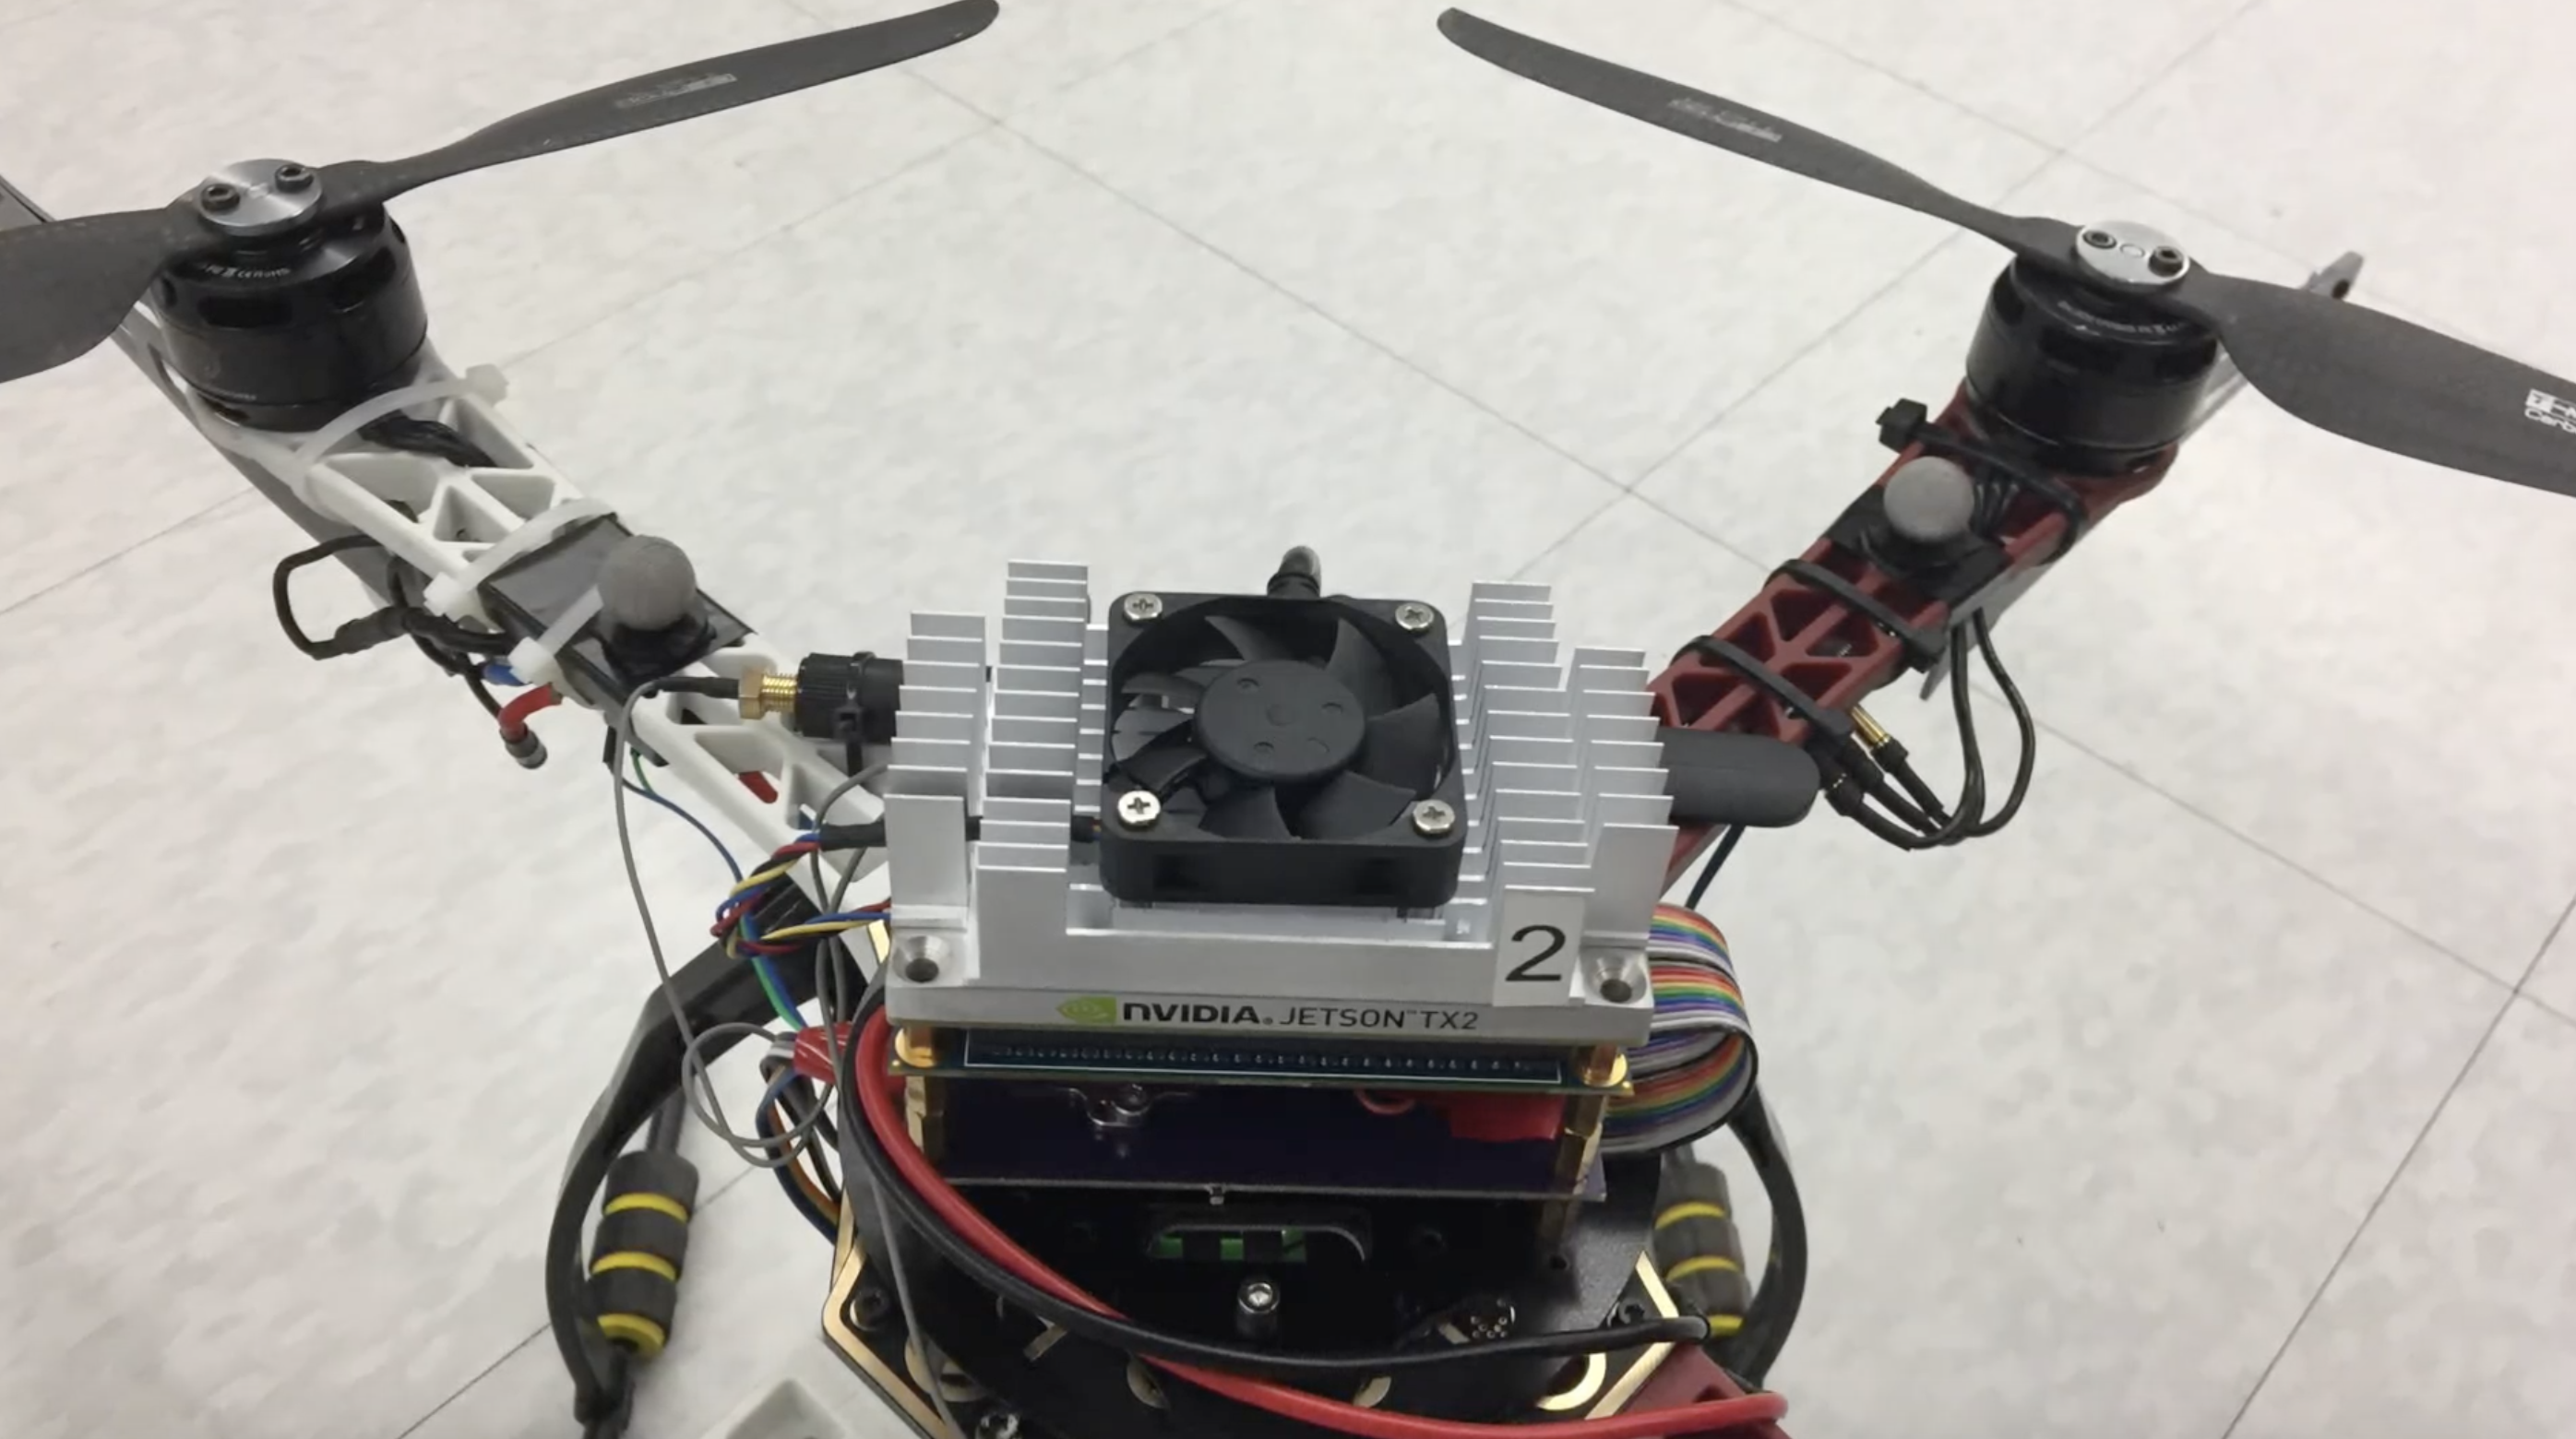
\includegraphics[width=\textwidth]{quad_top.png}
        		\caption{Quadrotor Top}
    	\end{subfigure}
	\hspace*{0.05\columnwidth}
    	\begin{subfigure}[t]{0.44\columnwidth}
           	\centering
          	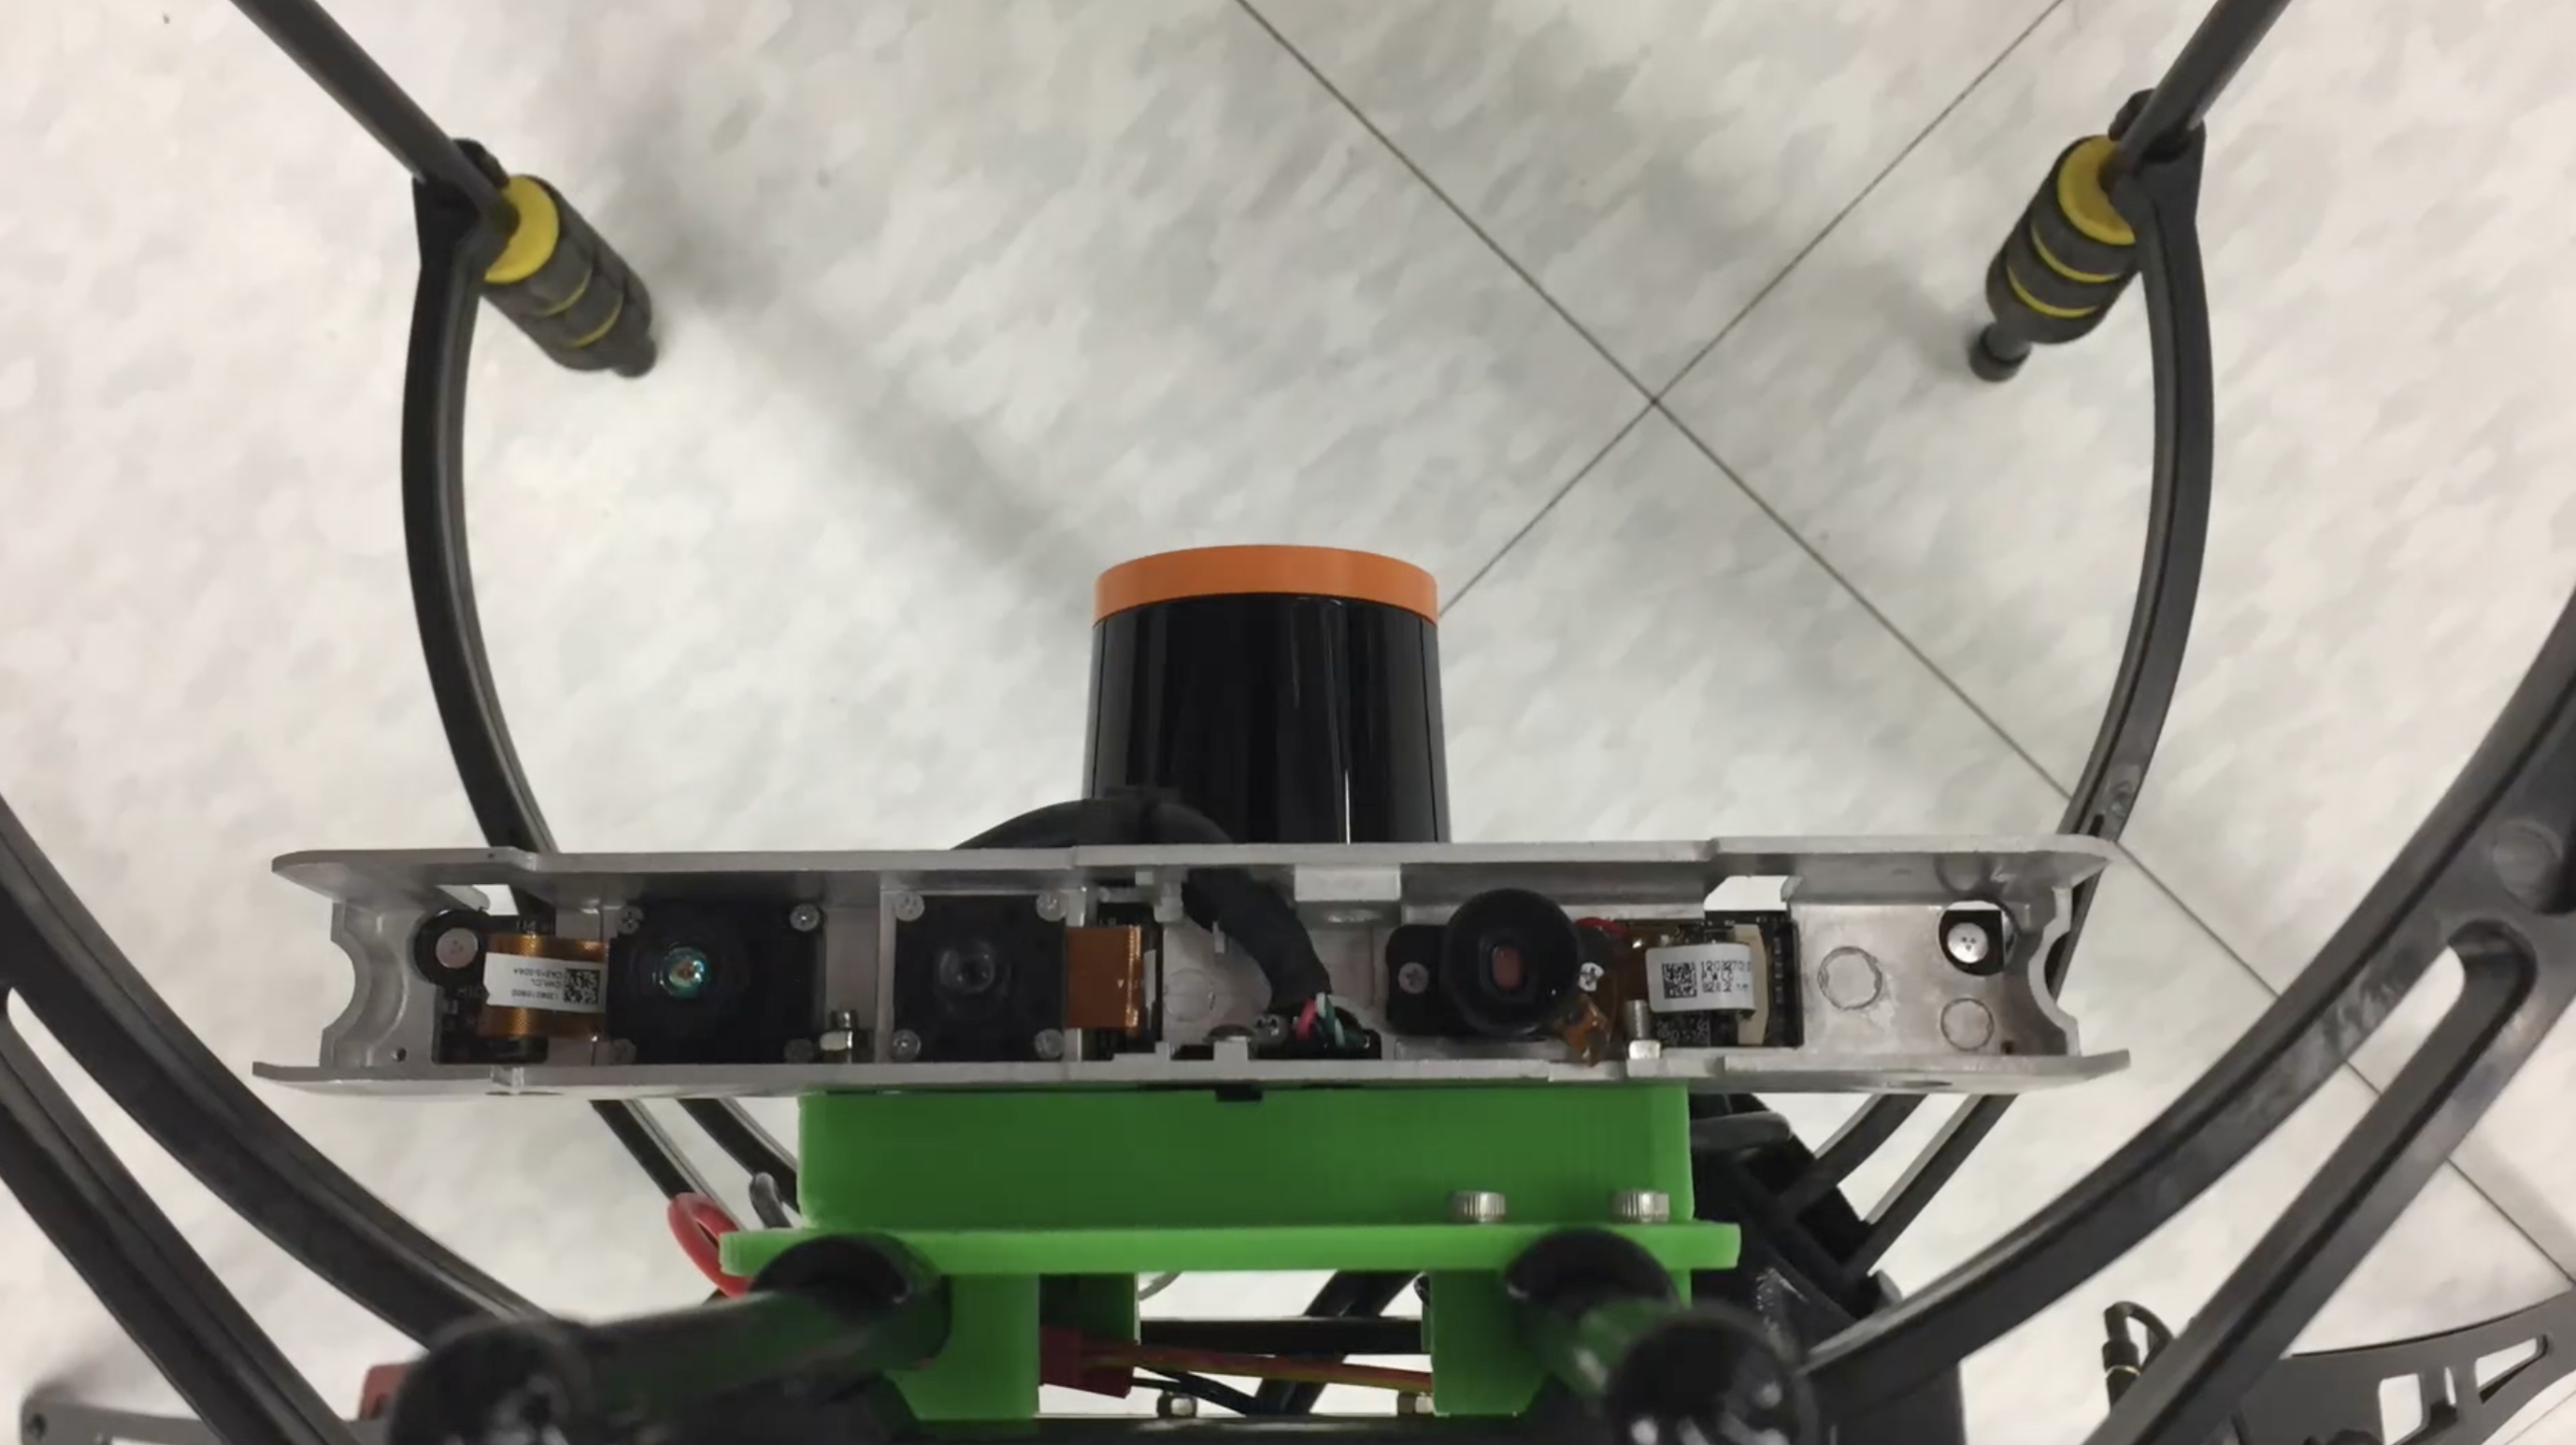
\includegraphics[width=\textwidth]{quad_bottom.png}
        		\caption{Quadrotor Bottom}
    	\end{subfigure}
	\caption{A Jetson TX2 (quadrotor top) streams depth measurements via WIFI from an Asus Xtion and Hokuyo LIDAR (quadrotor bottom). The host computer builds a 3D probabilistic occupancy grid map from these measurements. For autonomous exploration, the host computer designs exploration trajectories, which an onboard flight controller can track in real-time.}
	\label{fig:QuadrotorHardware}
\end{figure}

\subsection{Experimental Results}
                
The quadrotor takes off, completes a rotation to understand its immediate surroundings, then explores the space over $2$ minutes and $47$ seconds. Figure \ref{fig:exp3DMap} shows the probabilistic 3D map generated in real-time at four selected times, and the corresponding 2D projected maps (x-direction upward) are illustrated in Figure \ref{fig:exp2DMap}, where arrows represent pose candidates and a trajectory is shown to the optimal pose. Figure \ref{fig:expH} shows the total map entropy decreasing over the experiment duration. A video of the experiment can be found at \href{https://www.youtube.com/watch?v=I_1rXV2XRqk}{\WriteBlue{https://www.youtube.com/watch?v=I\_1rXV2XRqk}}.

% trim={<left> <lower> <right> <upper>}

\begin{figure}[!t]
\centering
    	\begin{subfigure}[t]{0.65\columnwidth}
           	\centering
          	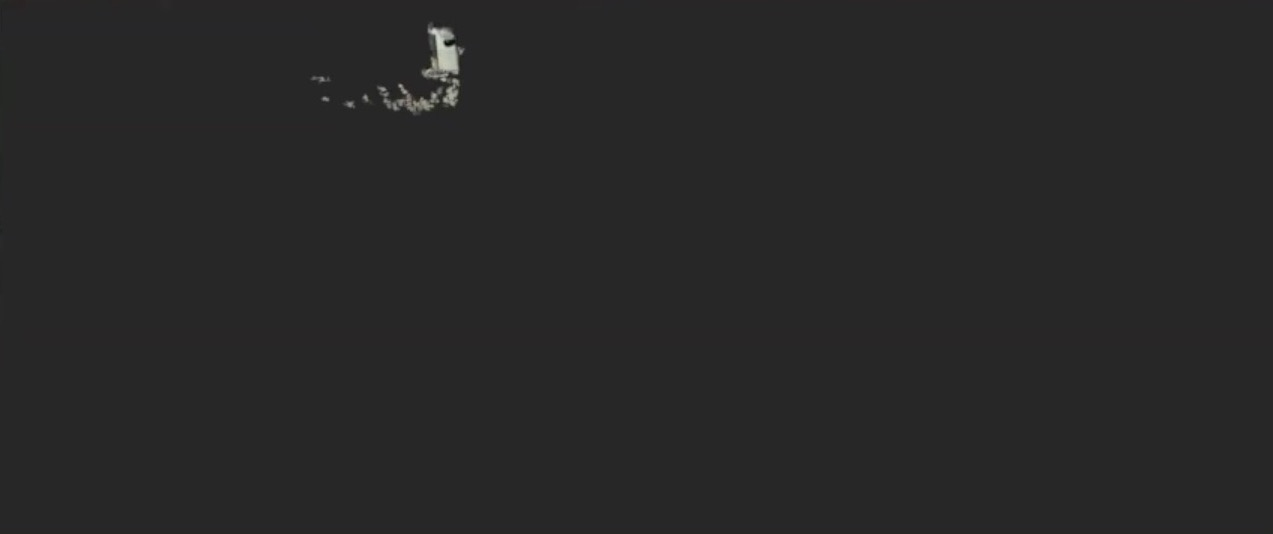
\includegraphics[width=\textwidth]{experiment_ogm3D_0min.jpg}
        		\caption{$0$ min}
    	\end{subfigure}
    	\begin{subfigure}[t]{0.65\columnwidth}
		\vspace*{0.01\columnwidth}
           	\centering
          	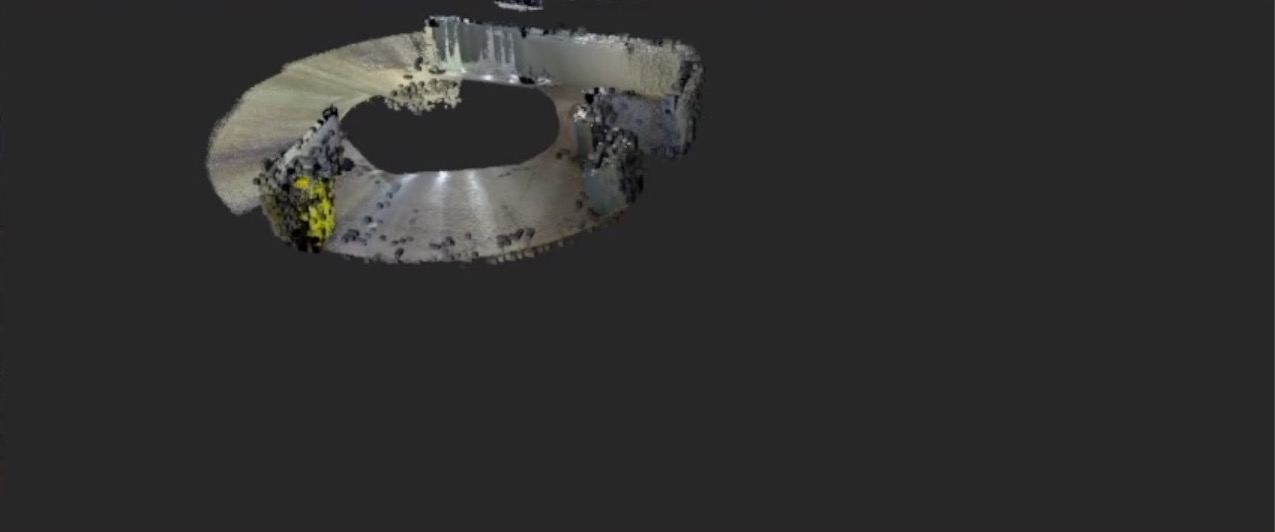
\includegraphics[width=\textwidth]{experiment_ogm3D_1min.jpg}
        		\caption{$1$ min}
    	\end{subfigure}
    	\begin{subfigure}[t]{0.65\columnwidth}
	\vspace*{0.01\columnwidth}
           	\centering
          	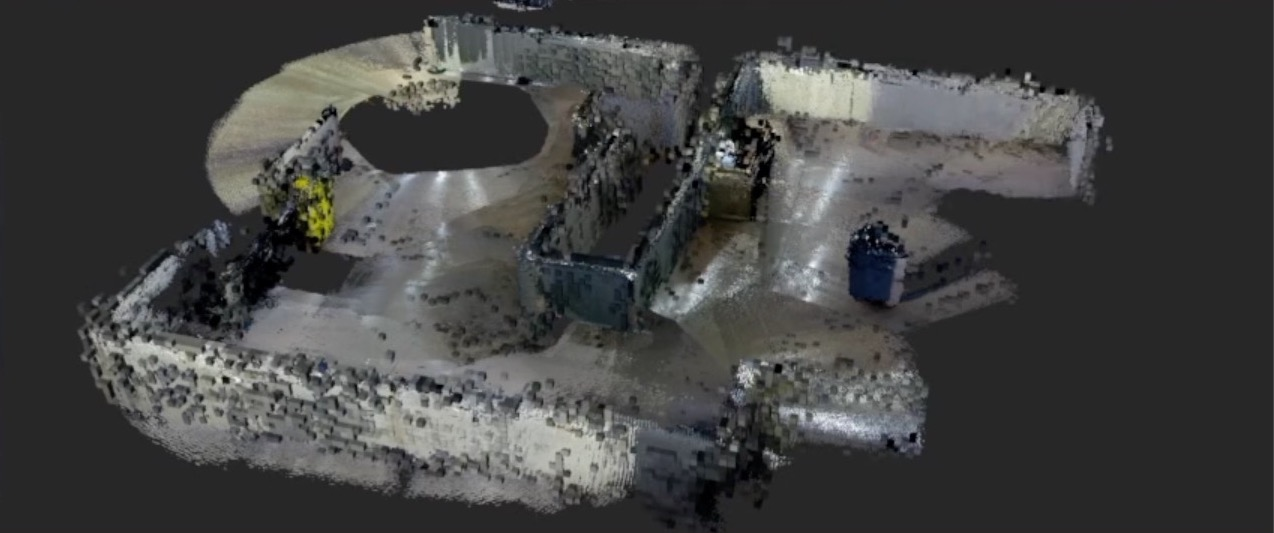
\includegraphics[width=\textwidth]{experiment_ogm3D_2min.jpg}
        		\caption{$2$ min}
    	\end{subfigure}
    	\begin{subfigure}[t]{0.65\columnwidth}
	\vspace*{0.01\columnwidth}
           	\centering
          	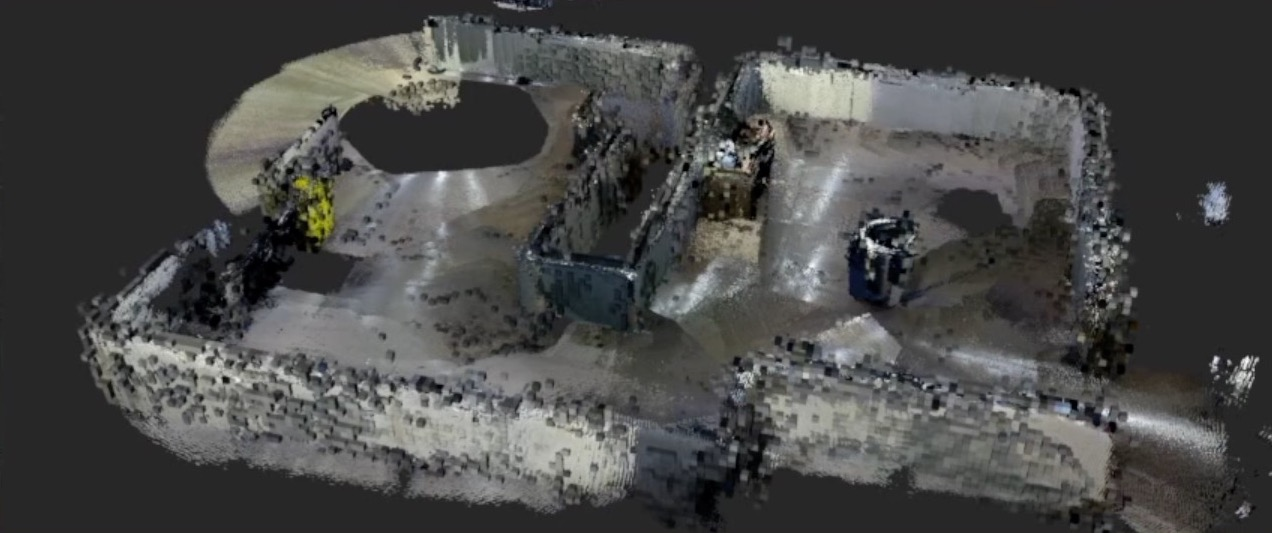
\includegraphics[width=\textwidth]{experiment_ogm3D_2min47sec.jpg}
        		\caption{$2$ min $47$ sec (end)}
    	\end{subfigure}
	\caption{The 3D occupancy grid map is overlaid with point cloud measurements. The map probabilities directly rely on the Xtion and Hokuyo measurements and the sensor stochastic properties.}
	\label{fig:exp3DMap}
\end{figure}

\begin{figure}[!t]
\centering
    	\begin{subfigure}[t]{0.44\columnwidth}
           	\centering
          	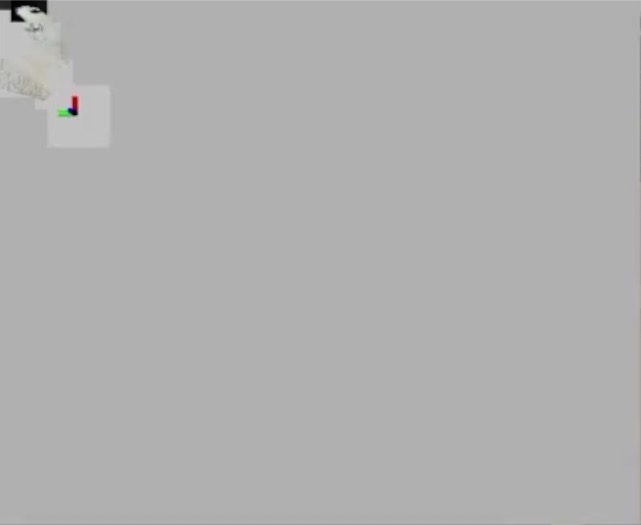
\includegraphics[width=\textwidth]{experiment_0min_2D.jpg}
        		\caption{$0$ min}
    	\end{subfigure}
    	\begin{subfigure}[t]{0.44\columnwidth}
           	\centering
          	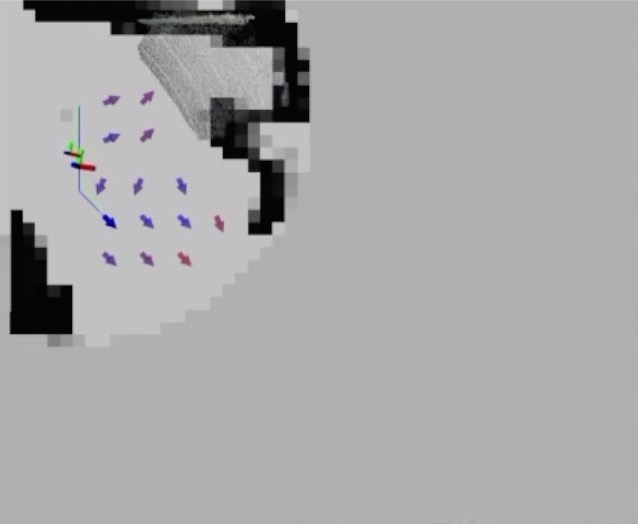
\includegraphics[width=\textwidth]{experiment_1min_2D.jpg}
        		\caption{$1$ min}
    	\end{subfigure}
    	\begin{subfigure}[t]{0.44\columnwidth}
           	\centering
          	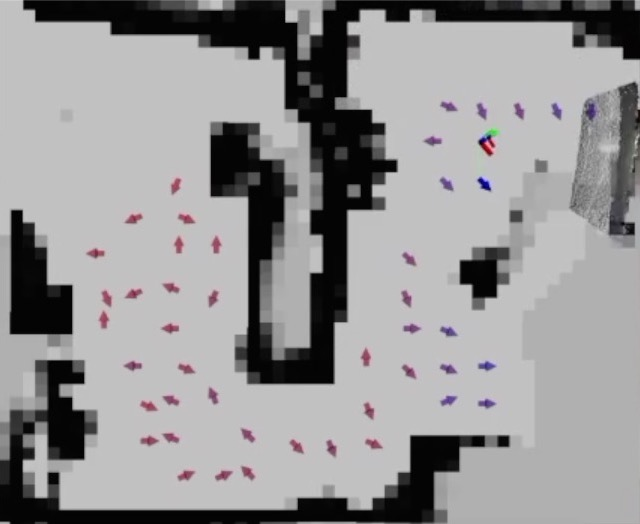
\includegraphics[width=\textwidth]{experiment_2min_2D.jpg}
        		\caption{$2$ min}
    	\end{subfigure}
    	\begin{subfigure}[t]{0.44\columnwidth}
           	\centering
          	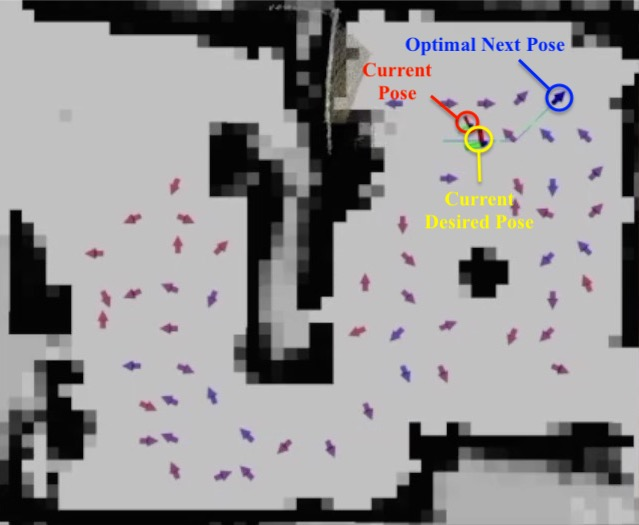
\includegraphics[width=\textwidth]{experiment_2min47sec_2D_labeled.jpeg}
        		\caption{$2$ min $47$ sec (end)}
    	\end{subfigure}
	\caption{The 2D projected map is easily produced in real-time. Candidate future poses, shown by arrows, have more blue color for larger objective functions, found with expected information gains and travel distances. Collision-free waypoints (blue line) serve as input to a constrained polynomial least-squares path (light green curve) for the robot controller to follow, where the desired pose (large axes) is tracked by the onboard controller from the current robot pose (small axes).}
	\label{fig:exp2DMap}
\end{figure}

\begin{figure}[!t]
	\centering
	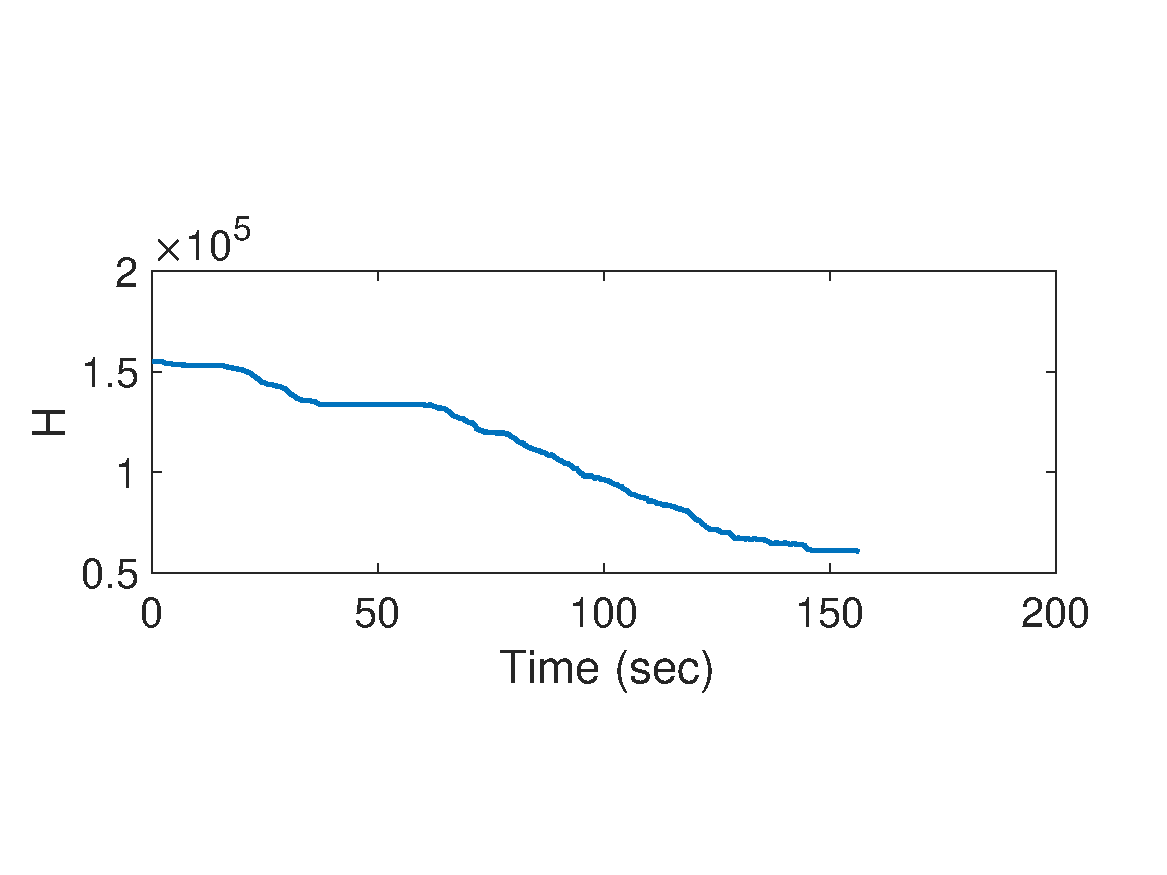
\includegraphics[width=0.85\textwidth]{entropy_experiment_aspect3by1.pdf}
	\caption{Map entropy decreases as the robot explores and captures more of the experimental environment.}
	\label{fig:expH}
\end{figure}

The robot is able to produce a 3D occupancy grid in under $3$ minutes without a human providing a trajectory. The 3D map can be easily interpreted by a human, and provides sufficient information in real-time for autonomous exploration. Optimal poses and collision-free exploration trajectories are calculated by the exploration node in under $1$ second. These quick decisions are vital to the autonomous exploration performance since the map is initially uncertain.

The projected map used for both collision and exploration has several benefits. The robot measures walls and objects with the 3D map, and nicely represents these as occupied spaces with the 2D projected map. Additionally, the exploration computation is low, allowing only for brief hover periods (less than $1$ second) between trajectories. However, the robot exploration does not consider those cells far below the robot, particularly those near the ground. As a result, some floor regions are not captured by the 3D occupancy grid even though cells above the floor are well-known. These neglected cells on the floor motivate the full 3D exploration, shown in the next experiment.



\section{Full 3D Exploration with a Quadrotor}
\label{sec:QuadrotorSEH}

In this final experiment, we introduce the quadrotor to a space with complex 3D objects. The robot generates a 3D map of this space, and performs autonomous exploration while considering the expected information gains of sample measurement rays with nonzero vertical components. The robot unlike prior examples, the robot also moves vertically during exploration and tracks the ground below the vehicle.

\subsection{3D Exploration Setup and Paramaters}
The software follows the same structure as in Section \ref{sec:MarsSimulation}, except the Gazebo simulated environment is replaces with experimental equipment. This equipment is identical to the prior experimental example (Section \ref{sec:QuadrotorNRL}), except the experiment took place at the Flight Dynamics and Control Lab (FDCL) inside the second floor of SEH. This environment is smaller with only $6$ cameras, where the x-direction (positive east) spans $-2.0$ m to $2.0$ m, the y-direction (positive north) spans $-2.0$ m to $2.0$ m, and the z-direction (positive vertically up) spans $-0.15$ m to $1.5$ m.


\subsection{3D Exploration Results}




